%-----------------------------------------------------------------------------
%
%               Template for sigplanconf LaTeX Class
%
% Name:         sigplanconf-template.tex
%
% Purpose:      A template for sigplanconf.cls, which is a LaTeX 2e class
%               file for SIGPLAN conference proceedings.
%
% Guide:        Refer to "Author's Guide to the ACM SIGPLAN Class,"
%               sigplanconf-guide.pdf
%
% Author:       Paul C. Anagnostopoulos
%               Windfall Software
%               978 371-2316
%               paul@windfall.com
%
% Created:      15 February 2005
%
%-----------------------------------------------------------------------------


\documentclass[preprint,numbers,10pt]{sigplanconf}

% The following \documentclass options may be useful:

% preprint      Remove this option only once the paper is in final form.
% 10pt          To set in 10-point type instead of 9-point.
% 11pt          To set in 11-point type instead of 9-point.
% numbers       To obtain numeric citation style instead of author/year.

\usepackage{color}
\usepackage{listings}
\usepackage{amsmath} 
\usepackage{amssymb}
\usepackage{graphicx}
\usepackage{array}
\usepackage{booktabs}
\usepackage{tabularx}

\definecolor{light-gray}{gray}{0.90}
\definecolor{dark-gray}{gray}{0.10}
\definecolor{dark-blue}{rgb}{0,0.08,0.45}
\definecolor{dark-green}{rgb}{0,0.50,0}
\definecolor{comment-green}{rgb}{0,0.4,0.1}
\definecolor{type-blue}{rgb}{0.16,0.56,0.68}
\definecolor{keyword-blue}{rgb}{0,0.2,0.7}
\definecolor{string-purple}{rgb}{0.59,0,0.57}
\definecolor{orange}{rgb}{1,0.5,0}

\def\codestyle{\color{black}\small\sffamily\upshape}
%\def\kwstyle{\codestyle\color{dark-blue}}
\def\kwstyle{\codestyle\bfseries}
%\def\tpstyle{\codestyle\color{type-blue}}
\def\tpstyle{\codestyle\itshape}
\def\idstyle{\codestyle}
%\def\commentstyle{\codestyle\rmfamily\color{comment-green}}
\def\commentstyle{\codestyle\rmfamily\color{comment-green}}

\newcommand{\textkw}[1]{\mbox{\kwstyle #1}}
\newcommand{\textcode}[1]{\mbox{\codestyle #1}}
\newcommand{\textid}[1]{\mbox{\idstyle #1}}
\newcommand{\texttp}[1]{\mbox{\tpstyle #1}}
\newcommand{\textcomment}[1]{\mbox{\commentstyle #1}}

\lstset{language=Java
       ,columns=fullflexible
       ,basicstyle=\codestyle
       ,literate={<<}{$\langle$}1 {>>}{$\rangle$}1 {<>}{$\neq\;\,$}1 {>=}{$\geqslant\;$}1 {\&\&}{$\wedge\;\,$}1 {||}{$\vee\;\,$}1 {++}{\texttt{++}}2 {;}{\,;}1 {xx}{$\times\;$}1 {^}{\ $\cdot$\ }2 {->}{$\rightarrow\;$}2 {NN}{$\N$}1 {~>}{$\rightharpoonup\;$}2 {=>}{$\Rightarrow\;$}2
       ,keywordstyle=\kwstyle
       ,emph={String,Bool,Int,Set,%
              int,string,timestamp,bool,str,void,set,map,time}
       ,emphstyle=\tpstyle
       ,identifierstyle=\idstyle
       ,tabsize=2
       ,commentstyle=\commentstyle
       ,keywords={entity,array,property,state,relation,function,var,orderby,match,with,not,global,%
                  where,select,do,sync,flush,yield,barrier,delete,max,min,sum,merge,entries,all,%
                  class,if,else,while,catch,await,return,delegate,foreach,in,try,finally,static,threadlocal,private,public,atomic,assert,ref,true,false,with,struct,method,type,const,null,%
                  cloud,table,grain,parallel,index,op,var,and}
       ,delim=[l][\upshape]()
       ,escapeinside={\%}{\%}
       ,stringstyle=\color{string-purple}
       ,showstringspaces=false
       ,morestring=[b]'
       ,comment=[l]//
       ,numbers=left
       ,numberstyle=\tiny
       }
\newcommand\comment{\commentstyle\quad// }
\newcommand{\hidden}[1]{}
\newcommand{\lref}[1]{line~\ref{l:#1}}
\newcommand{\rref}[1]{lines~\ref{b:#1}--\ref{e:#1}}

\newcommand{\mypar}[1]{\vspace{.05in}

\noindent\textbf{\textit{#1.}} }

\begin{document}

\special{papersize=8.5in,11in}
\setlength{\pdfpageheight}{\paperheight}
\setlength{\pdfpagewidth}{\paperwidth}

\conferenceinfo{PLDI '17}{Month d--d, 20yy, City, ST, Country}
\copyrightyear{20yy}
\copyrightdata{978-1-nnnn-nnnn-n/yy/mm}
\copyrightdoi{nnnnnnn.nnnnnnn}

% Uncomment the publication rights you want to use.
%\publicationrights{transferred}
%\publicationrights{licensed}     % this is the default
%\publicationrights{author-pays}

%\titlebanner{banner above paper title}        % These are ignored unless
%\preprintfooter{short description of paper}   % 'preprint' option specified.

\title{Reactive Computations for Distributed Actors}
\subtitle{}

\authorinfo{Sebastian Burckhardt}
           {Microsoft Research}
           {sburckha@microsoft.com}
\authorinfo{Tim Coppieters}
           {Vrije Universiteit Brussel}
           {coppieters.tim@gmail.com}

\maketitle

\begin{abstract}
Many online applications connect users in real-time, be it for games, social interactions, or collaboration. However, architecting services to power these applications while providing scalability, elasticity, fault tolerance, and low cost is difficult. To simplify this task, we propose \emph{reactive computations}, an extension of the virtual actor programming model. A reactive computation computes a result not once, but continuously - the runtime automatically detects dependencies and propagates changes, using a fault-tolerant distributed algorithm. Our cloud experiments show that reactive computations perform competitively compared to alternatives like explicit change propagation or polling. 
\end{abstract}

\category{CR-number}{subcategory}{third-level}

% general terms are not compulsory anymore,
% you may leave them out
\terms
term1, term2

\keywords
keyword1, keyword2

\section{Introduction}

Applications that run on client devices and cloud services are ubiquitous today. Since the early days of the internet, such applications have evolved from simple page-delivery engines to distributed reactive applications that let users share the experience and interact socially. Whether it is about games, collaborative editing, or online conversations: connecting users in real-time via a scalable and fault-tolerant service remains a significant and exciting challenge.

\mypar{Reactive Programming} Research on reactive programming has proposed many interesting solutions, and the community has been experimenting with many programming languages, language extensions, and frameworks. Simply speaking, a reactive programming model combines (1) a convenient way to express a view of some state or event source, and (2) a corresponding efficient mechanism that can update the view in response to state updates or events. It is a rich design space including many different philosophies and implementations. 

For example, in \emph{functional-reactive programming (FRP)}, we express views as signals that depend on event streams, and define them using a vocabulary of functional operators or combinators \cite{frp-firstprinciples,frp-animation,frp-frtime,elm,afp}. Another approach, which we call \emph{model-view computation}, is to define views as the result of a computation (functional or imperative) that depends on the model state \cite{alive,react}. In either case, propagating small changes selectively and efficiently is key. This can be achieved not only using FRP-style language support, but (alternatively or additionally) by runtime algorithms (such as virtual DOMs \cite{react,alive}, one-way dataflow constraints \cite{camil}, or self-adjusting computation \cite{acar-ahmed-blume-POPL08}) that can isolate which parts of a computation need to be updated in response to a change.

An important difference is that with FRP, all intermediate values matter (streams must not lose events), while for model-view computation, only the latest state of the model is relevant for computing the view. This distinction gains relevance when considering fault tolerance.

\mypar{Actor-Based Cloud Services} Much research has focused on reactive programming for graphical user interfaces \cite{elm,flapjax,alive} on the client. But often, the observed state or events are located not on the client, but in the service. Providing a reactive programming model for services is much harder than for a single machine. Performance is more elusive because of the high communication latency between machines. Moreover, a good service provides \emph{elastic scalability} (runs on a cluster that can be grown or shrunk at runtime),  \emph{fault tolerance} (automatically handles individual server failures) and \emph{compute-storage separation} (persists application data in a separate cloud storage system), 
% Not sure if you want to mention this like this, but I do think we should mention the current distributed reactive systems and their lacking in some way %
all of which are not guaranteed by the current distributed reactive models \cite{drescala}.

\emph{Actors} have emerged as a viable model for developing such services, because they can be distributed over a cluster \cite{erlang,akka,orleans}. In particular, \emph{virtual actor} runtimes \cite{orleanstr,orleans,sfactors,orbit} provide the necessary distributed protocols for persistence, load balancing, and fault detection. But how can we support reactive programming on virtual actor systems?
 
A common ad-hoc solution is to employ some sort of \emph{observer pattern}. The programmer takes full responsibility for tracking dependencies and propagating changes between actors. But even for non-distributed programs, observer patterns can lead to complex and error-prone code \cite{sobserver}; this only gets worse when we have to tolerate failures and provide persistence. 
%Clearly, more support from the language or runtime is desirable.

Another common approach is to add support for \emph{streams} \cite{orleans,reactors-io}. However, combining actors and streams can be confusing, as the FRP paradigm (state is an event stream) is at odds with the actor paradigm (state is encapsulated by asynchronously communicating actors). Also, it is difficult to make streams both fault tolerant and performant --- persisting every event is costly. 

\mypar{Reactive Computations} In this work, we propose a novel approach to distributed reactive programming that does not replace the actor paradigm, but extends it with a new feature called \emph{reactive computations}. Any client of the service can start such a reactive computation, which computes some result that depends on one or more actors of the service. But, as in self-adjusting computation \cite{Acar:SelfAdjustingOverview}, this result is computed not just once, but \emph{continuously}: the latest result is pushed to the client whenever it changes. 

Notably, the service code remains exactly the same ---  all the programmer has to do is to use a reactive computation on the client.  The reactive magic is not in the program, but in the runtime: it executes the computation in a special mode that intercepts all actor calls, including nested calls, and constructs a distributed dependency graph. Whenever the state of any actor involved in the computation changes, the change is automatically propagated, i.e. pushed along the edges of the dependency graph. This happens for as long as the reactive computation remains active. 

%Also, note that this computation is not restricted to a predefined vocabulary of operators, but can execute any code of the host language (imperative or functional). It does not require static analysis, but can call any number of dynamically determined actors, sequentially or in parallel. 

\mypar{Contributions} We make the following contributions:
\begin{enumerate}
\item We propose a new programming model for reactive elastic services, which extends the virtual actor model (\S\ref{sec:virtualactors}) with runtime support for reactive computations (\S\ref{sec:formulation}). 
\item We present a new fault-tolerant distributed reactive caching algorithm (\S\ref{sec:algorithm}), and implement it as an extension of the Orleans virtual actor runtime (\S\ref{sec:implementation}).
\item We provide a performance evaluation (\S\ref{sec:evaluation}) that demonstrates that the latency and throughput of our automatic change propagation compares favorably with alternative solutions, such as manual change propagation and polling.
\end{enumerate}    
   
\hidden
{
oncern.s between consistency and performance, and question of trading  choice to make highly depends on the circumstancesand may choose use explicit timeSynchronous vs. asynchronous, glitches, 
 
This structure can lead to specialized solutions (for example, the database community has known for decades how to solve the view-update problem for relational data). helps to implement efficient algorithms  to the view-update problem. Recursion is common, where views become subjects of other views: for example, signals in FRP can be defined in terms of other signals. Semantics can differ in how they treat 


use relations, may be monolithic, or graphs of objects. For example, database Facebook react has 
relationship, and how changes are propagated by the runtime. Prior approaches to reactive programming fall into two camps: explicit (the programmer expresses dependencies) and implicit (program expresses the viewdependencies are detected automatically, either at compile-time or at runtime).
Examples of explicit: makefiles, Rx, FRP. Examples of implicit: self-adjusting computation, Facebook React.

Philosophical: Model-View separation, Event Streams

  is has focused on specifying dataflow explicity. However, there are some 
}


\section{Virtual Actor Model}\label{sec:virtualactors}

Actors have emerged as a useful abstraction for the middle tier of scalable service applications that run on virtualized cloud infrastructure in a datacenter . In such systems, each actor is an object with a user-defined meaning, identity, state, and operations. For example, actors can represent user profiles, articles, game sessions, devices, bank accounts, or chat rooms. Actors resemble miniature servers: they do not share memory, but communicate asynchronously, and can fail and recover independently. One of the main benefit of actor systems is that they \emph{scale horizontally}, because the actor instances can be distributed across a cluster of servers.

In a traditional bare-bones actor system, the developer remains responsible for the creation, placement, discovery, recovery, and load-balancing of actors. A newer generation of actor models \cite{orleans,orbit,sfactors}, called virtual actor models, automate all of these aspects. The developer specifies only (1) a unique key for identifying each actor, and (2) how to save and load the actor state to/from external storage, if persistence is desired. As virtual actor systems can activate and deactivate actors based on use, they strongly resemble distributed caches ["14"]["39"]["40"]["55"] and provide similar performance benefits. 

Following the terminology ["4"], we call the virtual actors \emph{grains}. For each grain type, the code defines a (1) key that identifies instances, (2)  fields that define the grain state, and (3) operations supported by the grain. The operations of a grain can read and modify the grain state, and can call operations on other grains, but cannot directly read or write the state of other grains (encapsulation). 
 
\subsection{Example: Chirper}

As a running example, we use a service called \emph{Chirper} (based on the Orleans sample with the same name). It models a typical social application where users post messages to their own timeline, and view a timeline containing all messages posted by people they are following.
The code for the chirper service is shown in Fig.~\ref{fig:chirper}. We use imperative pseudocode and an imaginary actor DSL (domain-specific language) to focus on the programming model and minimize distractions (such as framework details or C\# language features). 

\begin{figure}
\begin{lstlisting}
grain User[userid: string] %\label{l:def}%
{
	// grain state
	state Messages: map<<time,string>>;%\label{l:msgs}%
	state Follows: set<<string>>;%\label{l:flws}%
	// update operations
	op Post(t: time, msg: string) { Messages[t] = msg; }%\label{b:uo}%
	op Unpost(t: time) { Messages.remove(t); }
	op Follow(id: string) { Follows.add(id); }
	op Unfollow(id: string) { Follows.remove(id); }%\label{e:uo}%
	// query operations
	op GetMessages(from: time) : list<<pair<<time,string>>>> { %\label{l:getm}%
		var msgs = new list<<pair<<time,string>>>>();
		foreach(var m in Messages)
			if (m.key >= from)
				msgs.add((m.key, m.value));
		return msgs;
	}
	op GetTimeline(from: time): list<<pair<<time,string>>>> {%\label{l:gettl}%
		var msgs = GetMessages(from);%\label{l:loc}%
		parallel foreach(var f in Follows) {%\label{l:par}%
			// retrieve messages from user f by remote call
			var fm = User[f].GetMessages(from); %\label{l:rcall}%
			foreach(var m in fm) { msgs.add(m); }%\label{l:add}%
		}
		msgs.sort();%\label{l:sort}%
		return msgs;%\label{l:ret}%
	}
}
\end{lstlisting}
\caption{Pseudocode for the Chirper service example.}\label{fig:chirper}
\end{figure}

There is only one type of grain, called \lstinline|User|.  A user grain encapsulates data associated with a user, and is identified by a string called \lstinline{userid} (\lref{def}). Each user grain stores the messages posted by that user in a map data structure \lstinline|Messages| (\lref{msgs}), keyed by timestamp. The current list of followed users is stored in \lstinline|Follows| (\lref{flws}). The grain state can change in response to update operations \lstinline|Post|, \lstinline|Unpost|, \lstinline|Follow|, \lstinline|Unfollow| (\rref{uo}) , which are invoked by the chirper client in response to clicking respective buttons.

The operation \lstinline|GetMessages(from)| (\lref{getm}) returns all messages by this user since the time indicated by \lstinline|from|; it straightforwardly computes the result by iterating over \lstinline{Messages}.  

The operation  \lstinline|GetTimeline(from)|  (\lref{gettl}) is more interesting. It returns a sorted list of all messages posted by the user \emph{and all followed users} since  the time indicated by \lstinline|from|. It computes the result as follows: first, it retrieves the locally stored messages (\lref{loc}). Then, \emph{in parallel} (\lref{par}), it calls \lstinline|GetMessages| on all followed users. These calls target other grains, by constructing a grain reference \lstinline|User[f]| to the grain for userid \lstinline|f| (\lref{rcall}). The returned messages are all added to the list \lstinline|msgs| (\lref{add}). After all the parallel tasks complete, the messages are sorted (\lref{sort}) and returned (\lref{ret}).

\subsection{Failure Model}

A grain may fail at any time, even when in the middle of executing an operation, and this can be observed by the application. The runtime does provide some support for simplifying the failure handling at the application level. 

\mypar{Recovery} If a grain is hosted on a server and that server fails, the runtime activates a fresh instance of the grain the next time it is accessed. 

\mypar{Persistence} Optionally, programmers can declare grains to be \emph{persistent}, which means their state is saved in external persistent storage. The state of a persistent grain is saved after each operation that updates the state, and loaded from storage when a grain is activated. The \lstinline|User| grains in the chirper example are persistent. 

\mypar{Timeouts} All grain operations throw a special timeout-exception if no response is received after a configurable time limit (the default is 30 seconds). This helps to avoid hangs and deadlocks at the application level if a grain fails before responding, or becomes unavailable for any reason.

If an operation times out, the caller does not know whether its effect was performed or not. To handle this issue, applications often design update operations to be \emph{idempotent} \cite{kapil}, so they can be safely retried after encountering a timeout-exception. For example, all the operations of the \lstinline|User| grain in Fig.~\ref{fig:chirper} are idempotent.

\section{Reactive Computations}\label{sec:formulation}

Suppose now that we want our chirper client to not just display a frozen snapshot of \lstinline|GetTimeline|, but to react to changes in the application state and refresh the user display accordingly. What are our implementation options? 

\begin{figure}
\begin{lstlisting}
while (interested) {
	try {
		var result = Grain[myuserid].GetTimeline();
		display(result);
	} catch(TimeoutException) { 
		display("server is not responding, retrying...");
	}  
	await delay(5000); // wait for 5 seconds between refresh
}
\end{lstlisting}
\caption{Possible solution using client-side polling.}\label{fig:polling}
\end{figure}

\subsection{Client-side Polling}\label{sec:polling}

 A straightforward solution is to call \lstinline|GetTimeline| periodically on the client to retrieve the latest state (Fig.~\ref{fig:polling}). This solution is easy to understand, requires no changes to the service code, and gracefully handles transient exceptions (such as caused by high load or server failures). However, it confronts us with a unpleasant tradeoff when choosing the \emph{polling frequency}: infrequent polling means the displayed result can lag significantly behind the latest result; but frequent polling dramatically increases the load on our service. We demonstrate this tradeoff experimentally in section \ref{sec:evaluation} .

\begin{figure}
\begin{lstlisting}
// new additions to  grain state
state Observers: map<<Observer,time>>; 
state Followers: set<<userid>>; 	
// new update operations
op AddFollower (userid: string)
	{ Followers.Add(userid); }
op RemoveFollower (userid: string)
	{ Followers.Remove(userid); }
op AddObserver (client: Observer, from: time)
   : list<<pair<<time,string>>>>{%\label{l:cs}%
 	Observers[client] = time; 
 	return GetTimeline(from);
}
op RemoveObserver (client: Observer)
	{ Observers.Remove(client); }
// modifications to existing update operations
op Post(tstamp: time, msg: string) { 
	...
	NotifyFollowers();  NotifyObservers();
} 
op Unpost(tstamp: time) { 
	...
	NotifyFollowers();  NotifyObservers();
}
op Follow(userid: string) {  
	... 
	User[userid].AddFollower(this.userid);
	NotifyObservers();
}
op Unfollow(userid: string) { 
	...  
	User[userid].RemoveFollower(this.userid);
	NotifyObservers(); 
}
// new propagation operations
op NotifyObservers() {
	foreach(var (client,from) in Observers) {
		var latest = GetTimeline(from);
		client.Notify(latest);
	}
}
op NotifyFollowers() {
	parallel foreach(var f in Followers) { f.NotifyObservers(); }
}
\end{lstlisting}
\caption{Cautionary sketch of what it may take to apply the observer pattern to the \lstinline|User| grain from Fig.~\ref{fig:chirper}.}\label{fig:observers}
\end{figure}

\subsection{Explicit Propagation}\label{sec:observers}

A more challenging, but possibly better-performing solution is to add code to our service that explicitly tracks dependencies and pushes changes to the client. Fig.~\ref{fig:observers} shows a sketch of how we can apply the observer design pattern to the User grain (many other variations are possible). Clients can register themselves as observers (\lref{cs}), which means they receive notifications containing the latest result. Each grain  tracks observing clients and followers and notifies them. \emph{But this solution leaves much to be desired. } We have polluted the grain state with information about observers, and it is unclear whether this state should be persisted (and thereby pollute our storage as well) or not (and thereby cause issues when grains fail). Also, as written, changes are still not propagated very efficiently --- there remain many potential optimizations, and opportunities for introducing subtle bugs. 

\hidden
{\begin{itemize}
\item It is not clear if the client observers should be considered part of the normal grain state and persisted along with it. If observer lists are not persisted, they are lost on failures - but if they are persisted, we pay a performance price.
\item We are now saving redundant information in the user grains (\lstinline{Follows} and \lstinline{Followers} represent the same relation), and can observe inconsistencies  (the state of multiple grains is not saved atomically).  
\item Changes are not propagated selectively: a change notification forces the client to reexecute the entire query, even if only a small part of the computation is different.
\end{itemize}
}

\hidden{
Conceivably, a skilled programmer can solve all of these issues at the application level --- but in our experience, this is a road that leads to complex, error-prone code that is susceptible to deadlocks and subtle race conditions. There is a better way.
}


\begin{figure}
\begin{lstlisting}
var rc = CreateReactiveComputation(%\label{l:crc}%
									() => Grain[myuserid].GetTimeline()   	);
var resulttracker = rc.GetResultTracker();%\label{l:crt}%

while (interested) {%\label{b:pl}%
	try {
		var result = await resulttracker.NextResult();%\label{l:await}%
		display(result);
	} catch(TimeoutException) { 
		display("server is not responding, retrying...");
	}
}%\label{e:pl}%
\end{lstlisting}
\caption{Proposed solution: runtime support for reactive computations.}\label{fig:rcapi}
\end{figure}


\subsection{Automatic Propagation}\label{sec:reactive}

By adding support for reactive computations into the virtual actor runtime, we can spare the programmer considerable hassle, and let them benefit from an automatic, optimized distributed algorithm for dependency tracking and change propagation. 

We propose a novel API for reactive computations over virtual actors (Fig.~\ref{fig:rcapi}). It is purposefully similar to the client-side polling solution (Fig.~\ref{fig:polling}) and likewise does \emph{not require any changes to the service code}. 

First, the programmer creates a \emph{reactive computation} object (\lref{crc}), passing an anonymous function that describes the computation. This instructs the runtime to construct a dependency graph which continuously tracks the result of that computation and propagates changes via pushing, until the rc object is disposed.

To consume the results, the programmer simply creates a \emph{result tracker} object (\lref{crt}). The result tracker operates like an enumerator that produces both the initial result, and any successive changed results, when we call \lstinline|NextResult| (\lref{await}). %\footnote{to avoid potential confusion: note that the result tracker is \emph{not} an enumerator for the produced timeline; rather, each call to \lstinline|NextResult| returns the latest version of the \emph{entire} timeline.}
Note that the code in the loop (\rref{pl}) looks just like the client-side polling solution (Fig.~\ref{fig:polling}), and has the same failure and exception semantics, but we no longer need to specify an arbitrary polling delay --- instead, the loop simply waits for a new result to arrive, and then delivers it immediately. With compiler support for \lstinline|await|, as in C\# \cite{Bierman2012}, this is just as efficient as using callbacks, because the compiler constructs continuations that do not block the thread.

Exactly how the client processes the results is outside the scope of this work, and likely depends on the chosen client framework. For chirper  we used react.js; it lets us simply assign the result to the model, and automatically does the diffing.

%adding support for reactive computations into the virtual actor runtime, we can avoid the hassle of changing the application code, and  retain the elegant simplicity and well-defined failure handling of the client-side polling solution (Fig.\ref{}). Our proposed API is shown

%The reason is that the virtual actor model already provides us with a clean decomposition of computations and clear interception points (grain calls) that can be cached (memoized) and updated reactively. 
 


\begin{figure*}
\centering
\begin{tabular}{cc}
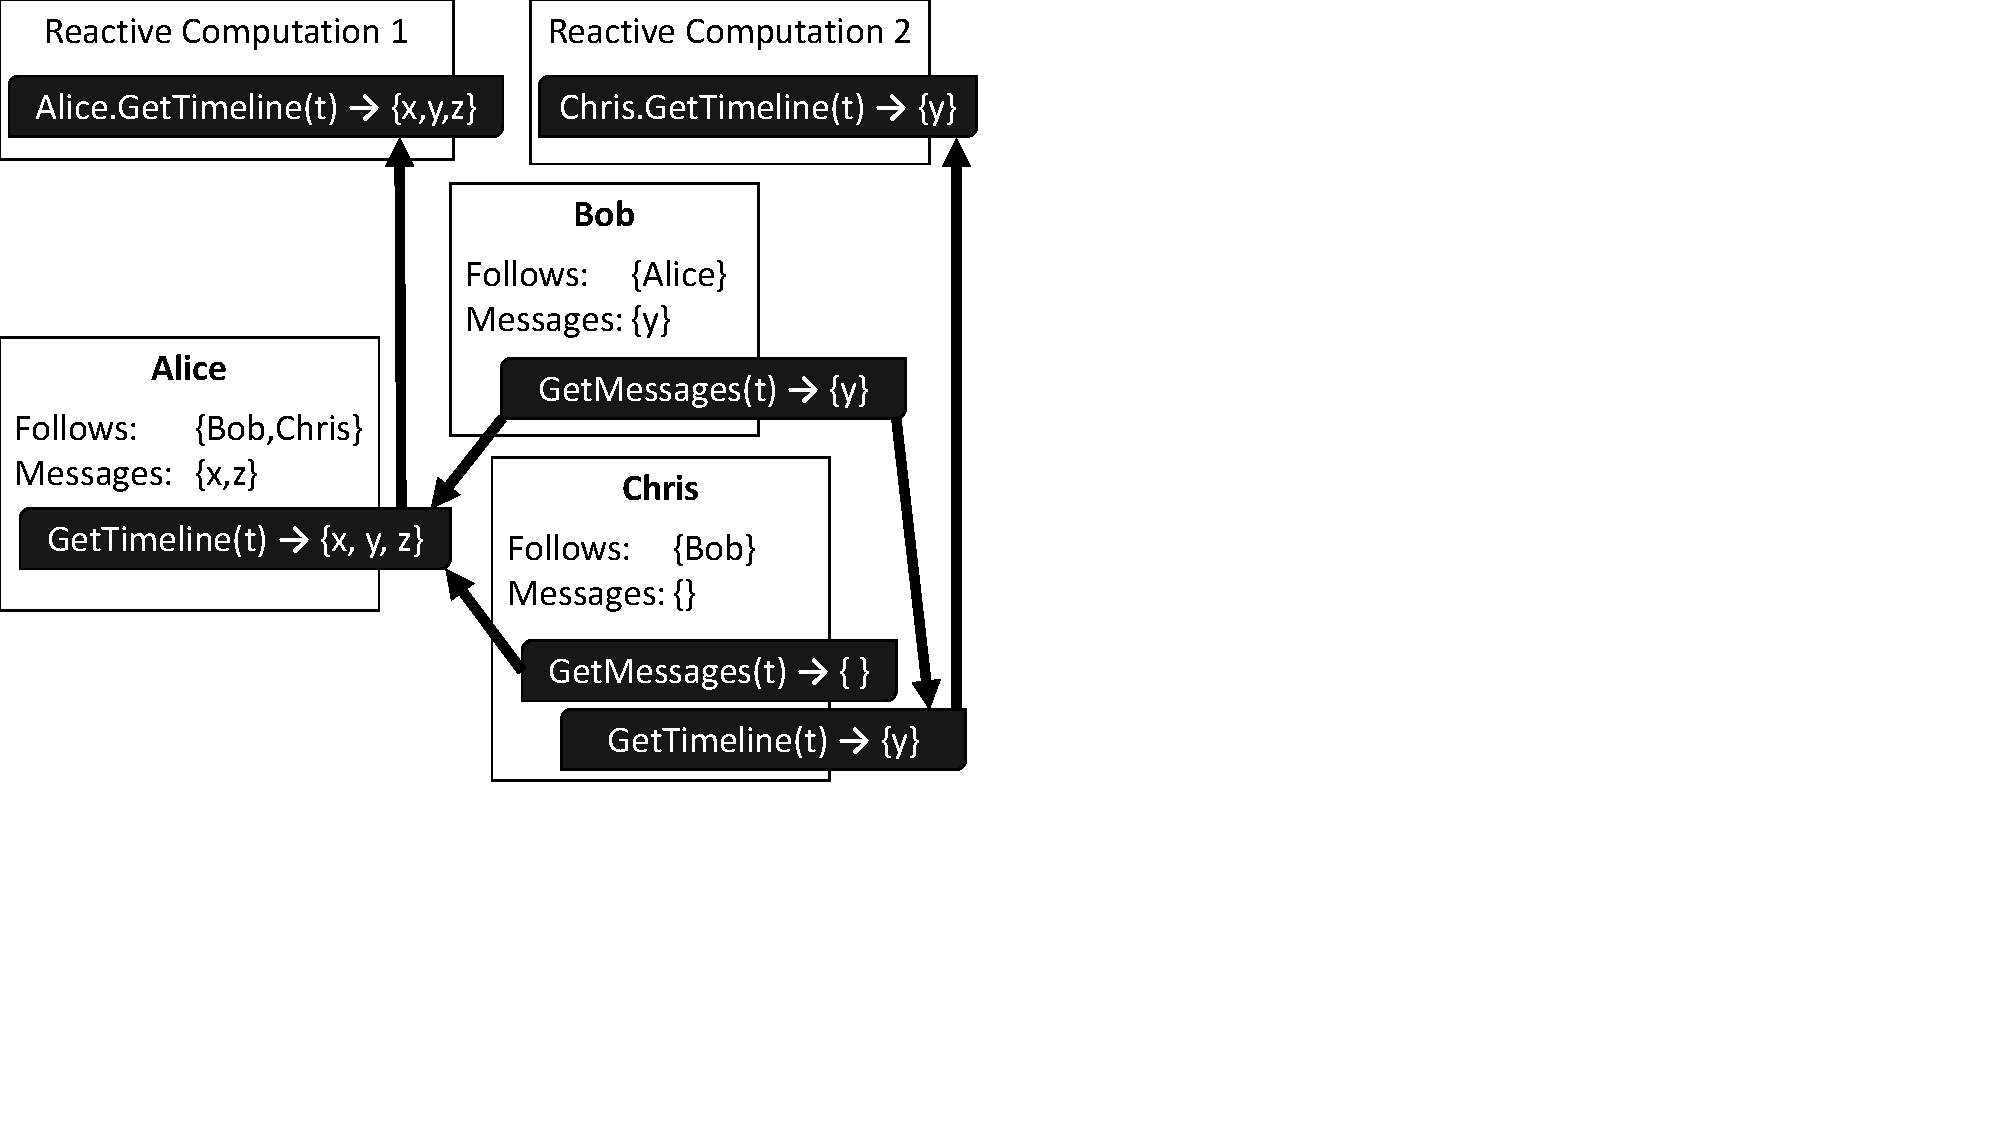
\includegraphics[scale=.45, viewport=-1 164 480 540]{figs/summaries}
&
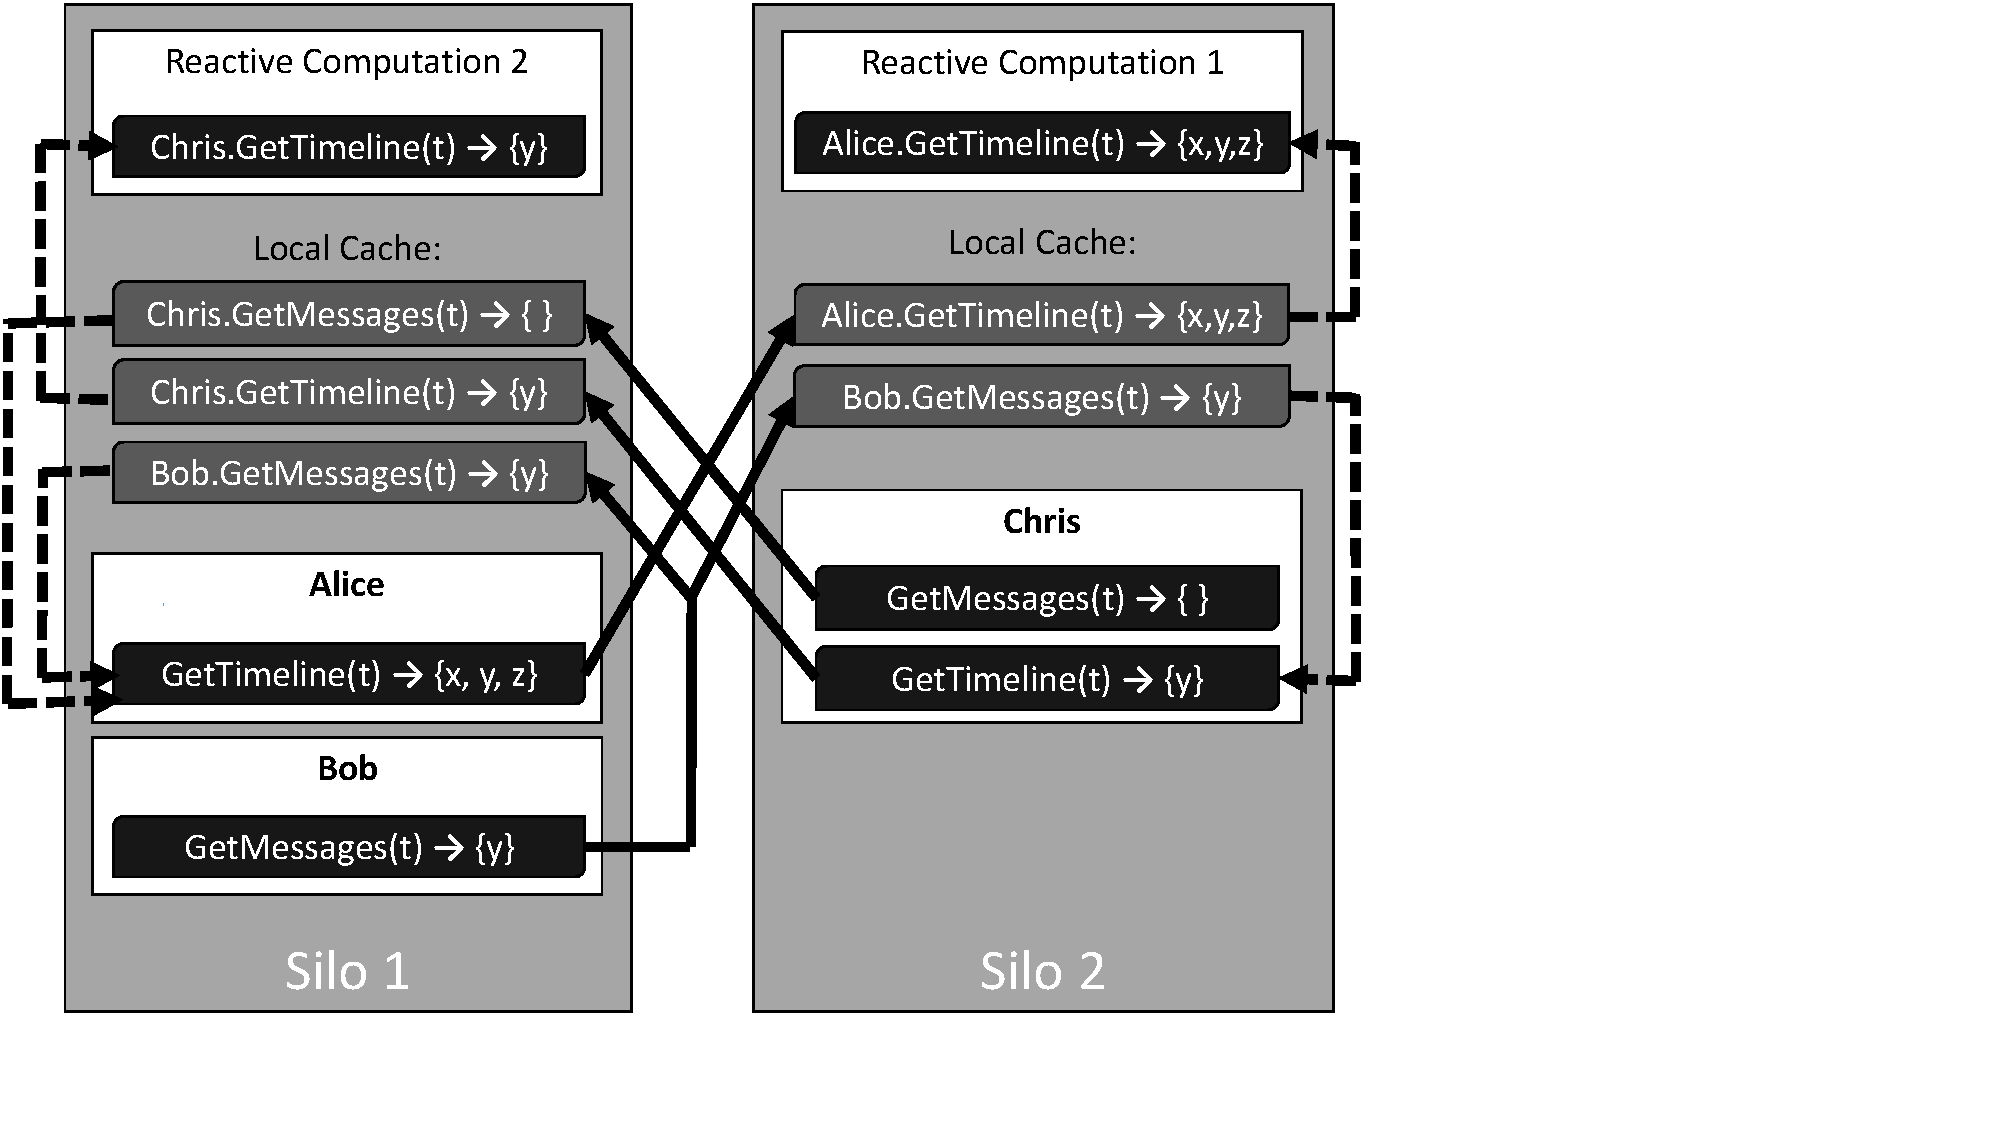
\includegraphics[scale=.4, viewport=-10 53 656 540]{figs/silos}\\
\end{tabular}
\caption{\textbf{(a)}  (on the left) example of a dependency graph of summaries, for two reactive computations; \textbf{(b)} (on the right) example of a corresponding bipartite dependency graph of summaries and local caches, distributed over two silos.}\label{fig:summaries}
\end{figure*}

\section{Algorithm: Reactive Caching}

To determine when a result of a reactive computation changes, we track all the grains it depends on. Tracking these dependencies is done entirely at runtime and does not require any static analysis: rather, we modify the virtual actor runtime to intercept grain calls and construct a \emph{dependency graph}.

We explain the dependency graph in two stages: first, we describe it as a directed ayclic graph of summaries (\S\ref{sec:summaries}). Then, we show to represent it as a bipartite graph of summaries and caches (\S\ref{sec:bp}) to improve performance and handle failures in a distributed setting. 

\subsection{Summaries and Dependencies}\label{sec:summaries}

During execution, we record and store a \emph{summary} for each executed operation. A summary is a pair consisting of (1) the invoked operation (including grain identity, method name, and all parameters), and (2) the value or exception returned at the end. For each summary, we record what other summaries it depends on, and what summaries depend on it. The result is a \emph{dependency graph} that represents the computation that was performed.

Fig.~\ref{fig:summaries}(a) shows an example of a dependency graph of summaries. Two clients perform reactive computations \lstinline|Alice.GetTimeline(t)| and \lstinline|Chris.GetTimeline(t)| for the same time parameter \lstinline|t|. Summaries are shown as black boxes, and reside either in a grain or in a reactive computation. Summary dependencies are shown as black arrows.

\mypar{Reuse} If a summary for a particular operation already exists, we reuse it. For example, \lstinline|[GetMessages(t)->{y}]| of Bob's grain is shared: two other summaries depend on it. 

\mypar{Re-execution} If a summary is stale (see \S\ref{sec:cp}), it is marked for re-execution. When re-executed, the dependencies may change, and are updated accordingly. 
%After a summary for a reactive computation is re-executed, we push the new result to the client.

\mypar{Garbage Collection} A summary for a grain method is deleted if there are no other summaries that depend on it.  A summary for a reactive computation is deleted when the reactive computation object is disposed. Since the dependency graph is acyclic (a cycle would represent a query with infinite recursion, which is prevented by the runtime), this means that summaries are guaranteed to be collected when no longer needed.  

\subsubsection{Change Propagation}\label{sec:cp}

We call a summary \emph{stale} if a re-execution of the computation or operation would necessarily yield a different result. Our change propagation algorithm guarantees that \emph{any stale summary is eventually re-executed}. Because grains cannot share any state, summaries can become stale for only two reasons: either (1) the state of their grain changes, or (2) a summary they depend on becomes stale. Thus, the following is sufficient:
\begin{enumerate}
\item Whenever a grain operation changes the state of a grain, we mark all summaries of that grain for re-execution.
\item After a summary for a grain operation is re-executed, we compare the new result to the previous result. If it is the same, no further action is needed. Otherwise, we mark all dependent summaries for re-execution.
\hidden{\item After a summary for a reactive computation is re-executed, we push the new result to the consuming result tracker object.}
\end{enumerate}
 
\noindent For example, executing the operation \lstinline|Chris.Unfollow("Bob")| will mark both of the summaries in Bob's grain for re-execution. Re-execution of \lstinline|[GetMessages(t)->{}]| yields the same result, and propagation stops. But re-execution of \lstinline|[GetTimeline(t)->{y}]| yields a different result \lstinline|{}|, which means we mark the dependent summary in Reactive Computation 2, \lstinline|[Chris.GetTimeline(t)->{y}]|, for re-execution. After it re-executes, the latest result reaches the client as desired.

\paragraph{Ephemeral Inconsistency. }  
%There are no guarantees about the relative consistency of summaries that are used in a computation (since we just use the most recent summary available for a given invocation). 
It is possible for the result of a computation to be inconsistent, in the sense that it is based on versions of grain states that never existed at the same time, or even on different versions of the same grain's state. However, if the result of a computation is inconsistent, then it is also ephemeral: an inconsistent summary must be stale, and is thus guaranteed to be re-executed and replaced.

\mypar{Batching} Some time may pass in between marking a summary for re-execution and the actual re-execution. In particular, it may be marked multiple times. This batching effect is important for maintaining good throughput under high update frequencies, as we demonstrate in the evaluation section.

\subsection{Reactive Caching}\label{sec:bp}

Under the hood, Orleans' virtual actor runtime load-balances grains across different physical machines called silos. The set of silos can change when administrators choose to increase or decrease the number of servers, or when servers fail (which is detected automatically). By design, the application layer is unaware of the existence of these silos. However, to make our algorithm performant and fault-tolerant, the spatial distribution of grains over silos is relevant, because (1) the latency of a remote call is orders of magnitude higher than the latency of a local call, and (2) silos can fail independently. Thus, we build an extra \emph{caching layer} into the dependency graph.

Rather than summaries that depend directly on other summaries, we now have summaries depend on local caches of summaries. Each summary maintains a connection to all its caches on the various silos, and pushes changes to those caches whenever a re-execution produces a different result. This \emph{reactive caching} mechanism improves performance because it can elide many slow remote accesses in favor of fast lookups in a silo-local hash table.

As an example, consider Fig.~\ref{fig:summaries}(b). It shows a bipartite graph of summaries and caches that corresponds to the dependency graph in Fig.~\ref{fig:summaries}(a). We show two types of edges: summary dependencies (dotted arrows), which are always within a silo, and cache connections (solid lines), which may cross silo boundaries. 

Extending change propagation and garbage collection to the bipartite graph is straightforward: when a cache receives a new value, it marks dependent summaries for re-execution. Caches are removed if they have no summaries that depend on them, and summaries are removed if they are not connected to any caches. 

\mypar{Fast Re-execution} When a summary is re-executing, and its dependencies have not changed, all of its grain operations hit in the local cache. Therefore, the overhead of re-execution of summaries is quite low: the latency of our change propagation mechanism is very close to the performance of a hand-written change propagation solution, as we demonstrate in the evaluation section.

\mypar{Large Fan-out} The reactive caching improves performance in situations with a large fan-out (summaries with many observers): rather than sending updates to each observer directly, it is enough to send one update to each silo, and the silo then forwards the update locally. This reduces network traffic.

\mypar{Back-Pressure} 
Our experiments show that in the case of high update rates, it is beneficial to throttle the sending of updates. Our mechanism achieves this by sending results to caches one at a time, and measuring the response time. If above a configurable threshold, we back off (wait for an extra delay equal to the round trip time of the push). 

\subsubsection{Fault Tolerance}

To tolerate faults, we need to make sure that we correctly handle the disappearance of any components that are visible to components on other silos.\footnote{we need not worry about components that are not visible on other silos, because whenever they fail, all components that are aware of them also fail.} In our case, the only thing we need to be concerned about is the connection between summaries and caches (this is readily apparent in Fig.~\ref{}: the only lines that cross silo boundaries are the solid edges).

Each summary maintains a list of connected caches. To maintain this connection, a cache periodically \emph{re-subscribes} every 30 seconds. This resubscription allows us to handle one-sided failures as follows:
\begin{itemize}
\item if a cache fails, it will no longer resubscribe. If a summary does not hear from a cache for 90 seconds, it removes it from the list. 
\item if a summary fails, the cache sends a resubscription after some time --- but the summary, and its associated grain, no longer exist. In that case, the standard virtual actor mechanism reactivates the grain on some silo, and loads its state from persistent storage. Then we recreate the summary and execute it. The cache is now connected to the new instance of the same summary. 
\end{itemize}

\section{Implementation} \label{sec:implementation}
There are a couple of interesting things to discuss with respect to our current implementation, even though they do not necessarily contribute to the core algorithm of this paper. In general, the actual C\# code is very similar to the pseudo-code used in this paper, but it contains more detail and uses language features that are not highly relevant in this context, albeit interesting in their own right (e.g. LINQ expressions, cooperative concurrency with async-await).


\paragraph{Detecting Changes.} The propagation algorithm described in \S~\ref{sec:cp} assumes that we can detect whenever the state of a grain changes. Even though that might be possible, we opted for a simpler approach and used a \textit{heuristic}: we assume that every method call that was not invoked in context of a reactive computation, might change the grain's state. By doing so we over-approximate the operations that might cause state changes. In the same vain that programmers have to indicate to the runtime when they want the state to be persisted (using a dedicated \texttt{WriteStateAsync()} method), we could in the future also provide a call that invalidates the grain's summaries. For persisted grains, we could even re-use the persistence call, since the programmer already clearly indicates significant state changes have been made.

\paragraph{Garbage Collection.} Even though the result of the reactive computation might not be required any more, the programmer might still be holding on to a reference of the reactive computation object, or even just a tracker. This would prevent the runtime from cleaning up the entire distributed dependency graph. In order to prevent this, we instruct the programmer to always create reactive computations and trackers within a C\# \texttt{using} block (as shown in Fig. \ref{fig:impl} Lines 1 and 3). This guarantees that the reactive computation is directly disposed when it's not used any more. Consequently, the bipartite graph will only exist, and thus produce overhead, as long as anyone is using it, giving the 90 second time frame for cleaning up.

% This Figure can easily be removed when the page limit is reached %%
\begin{figure}
\begin{lstlisting}
using(var rc = GrainFactory.CreateReactiveComputation(
									() => Grain[myuserid].GetTimeline())) {
	using(var resulttracker = rc.GetResultTracker()) {

		while (interested) {
			try {
				var result = await resulttracker.NextResult();
				display(result);
			} catch(TimeoutException) { 
				display("server is not responding, retrying...");
			} catch(DivisionByZeroException) {
				display("can't divide by zero");			
			}
		}
	}
}
\end{lstlisting}
\caption{Proposed solution, including the \texttt{using} constructs that make sure the graph is garbage collected when no longer required.}\label{fig:impl}
\end{figure}

\paragraph{Non-Determinism.}
Whenever a method is called from within the context of a reactive computation, it is now prone to being re-executed without the programmer explicitly performing the call. Furthermore, we assume that when such invocation is performed twice with the same grain state (and the grains it depends on), the result is the same. In other words, the algorithm disregards any other source of non-determinism such as clock queries and I/O. The programmer should thus avoid using these operations in a reactive computation. Keep in mind that this solution is geared towards performing some kind of \emph{query} over the distributed state, thus it makes sense to make this assumption. Currently, we do no statically or dynamically enforce this, because some type of non-deterministic operations might still be useful for example for debugging purposes. On the other hand, it might be interesting to explore extensions of the algorithm that do explicitly incorporate this by for example recording and re-using non-deterministic operations.

\paragraph{Exception Handling}
As can be seen from Fig.~\ref{fig:impl} (lines 11-13), whenever an exception occurs somewhere down the reactive computation, we don't simply stop the computation and deconstruct the dependency graph. Instead we assume the exception just occurred due to some current state of the grains, but following states might produce results again. The exception can be catched (1) either somewhere upstream in the reactive computation itself, or (2) on the \texttt{NextResult()} call of a tracker if it wasn't caught. This also provides a uniform way of handling both distributed exceptions (timeout) (Fig.~\ref{fig:impl} line 9) and computational exceptions (Fig.~\ref{fig:impl} line 13).


We have implemented reactive computations as extensions to Orleans, an open-source distributed actor framework for .NET available on GitHub ["37"]. The Orleans runtime already provides the needed distributed protocols for managing the creation, placement, discovery, recovery, and load-balancing of grains. What we added is (a) extensions to the grain objects to store summaries, (b) interception points for grain calls, (b) modifications to the grain scheduler to distinguish between reactive and normal execution mode, and (c) a silo-wide cache manager. 

In an object-oriented imperative language like C\#, we cannot statically determine whether a grain operation modifies the grain state. Thus, we conservatively trigger change propagation after \emph{any} operation on a grain. This is not as expensive as it may seem at first, because if the grain state has not changed, re-execution of the summary produces the same result, and propagation stops. Still, the programmer can annotate an operation as read-only to avoid this overhead; also, we assume that any operation called as part of a reactive computation does not change the grain state, and avoid summary re-execution in that case.

\hidden
{
\subsection{Runtime Implementation}

Under the hood, the runtime must provide the needed distributed protocols for managing the creation, placement, discovery, recovery, and load-balancing of actors. By design, the application layer is largely unaware of how these details. Nevertheless, we briefly describe the mechanisms used by the Orleans system here. 

\mypar{Grain Directory} Grains can be active (there exists an instance of it on some machine) or inactive (otherwise). The runtime maintains a distributed directory (based on the consistent hashing algorithm)  for tracking active grains. When an inactive grain is accessed, the runtime automatically activates it, and places it on a randomly selected server. If a grain is not accessed for a prolonged (configurable) time, it is deactivated and removed from the grain directory. 

\mypar{Silo Failures} Under the hood, the runtime tracks all participating servers, called \emph{silos}, using a membership protocol. The set of members can change when administrators choose to increase or decrease the number of servers, or when servers fail, which is detected automatically.  For \emph{volatile} grains, the grain state is lost on failure. For \emph{persistent} grains, the grain state is saved to persistent storage after each change, and loaded from persistent storage when activated. 
 

--- The actual C\# code is similar, but contains more detail and uses language features that are not highly relevant in this context, albeit interesting in their own right (e.g. LINQ expressions, cooperative concurrency with async-await).

--- ResultTrackers have some interesting properties that make them well suited for situations where updating the display requires I/O, such as when communicating with a remotely connected client device:   (1) result trackers may skip intermediate versions: only the latest result matters, and (2) result trackers return a task that can be efficiently awaited without blocking the thread (using C\# language support for async/await \cite{Bierman2012}).  Also, it is possible to use multiple result trackers for the same reactive computation, and each one can consume results at its own speed.

--- reactive computations available on silo or client
}


\section{Performance Evaluation}\label{sec:evaluation}

When operating a service, the overall performance objective is to provide acceptable service latency at minimal cost. The cost can be lowered by running fewer servers - but this increases the latency because requests spend more time waiting for contended resources (such as network, storage, CPU, threads, locks, and so on). This tradeoff is an essential challenge for developers writing an elastic service application. 

To clarify the value that our automatic, fault-tolerant change propagation provides to service architects, we now quantify both (a) its latency and (b) its resource consumption, by comparing them to alternative solutions, including periodic polling (\S\ref{sec:polling}), which is also fault-tolerant, and explicit change propagation at the application level (\S\ref{sec:observers}), which is not fault-tolerant. To this end, we designed two series of experiments that measure low-load latency (\S\ref{sec:latency}), and variable-load throughput (\S\ref{sec:throughput}).

\mypar{Application Model}  
We model the application using  \emph{item} grains that are observed by \emph{view} grains. Each view depends on a fixed number of items, selected at random at the beginning of the test. Views are updated when items change, in a manner that depends on the chosen propagation solution.
%, one of \emph{polling} (\S\ref{sec:polling}), \emph{explicit propagation} (\S\ref{sec:observers}), or \emph{automatic propagation} (\S\ref{sec:reactive}). 
Moreover, we vary the number of items and views to simulate different workloads (Table~\ref{tab:param}).  For example, a high \emph{fan-out} (= average number of views that depend on an item) means that whenever an item is mutated, many views need to be updated. 

The items and views run on five Orleans silos deployed as a Windows Azure cloud service. The robots run on 10 load generator servers. All processors have 8 cores, 14GB of RAM, and run at 1.6 GHz. To account for unexpected variations, we made sure to run each experiment series on at least 2 different datacenters, on at least 3 different days, and running the experiments in different order. Between runs, absolute numbers can vary up to 10\%, but the relative performance of the various solutions were stable. Note that we achieved this only after investing substantial work into our experimentation framework. 

Note that by design, this is a microbenchmark that isolates the mechanism we want to measure (change propagation) and removes all other aspects. If deployed as part of a complete service, including item persistence, the performance differences between the various solutions are likely to be less pronounced.
 
\begin{table}
\begin{tabularx}{.99\columnwidth}{@{}Xrrrr@{}} \toprule
Name		& \#items 	& \#views & \#deps. & max robots\\ \midrule
low-load	&  600        	& 20       & 4 & n/a \\
fanout-1	& 20,000	& 20,000 & 1& 2,000 \\
fanout-20	& 10,000	& 20,000 & 10 & 2,000\\
fanout-200 & 1,000	& 20,000 & 10& 1,000\\  
\end{tabularx}
\caption{Parameter combinations we used.}\label{tab:param}
\end{table}


\subsection{Latency}\label{sec:latency}

Our latency experiments use the low-load parameters (Table~\ref{tab:param}) to eliminate delays caused by queueing and contention. We measure two types, called \emph{query latency} and \emph{propagation latency}. Latencies are measured 4000 times each (200 times per view, separated by 500ms). We describe the results using the median and lower and upper quartiles.\footnote{Average and standard deviation are unsuitable statistics because of the long tail of the distribution.}

\subsubsection{Query Latency}

\begin{figure}
\begin{lstlisting}
grain View
{
	state Deps: Item[numdeps]; 
	op Query(sequential: bool) : int[]
	{	
		var result = new int[numdeps];
		if (sequential) {
			for (0 <= i < numdeps)
				result[i] = Deps[i].GetValue();
		} else {
			parallel for (0 <= i < numdeps)
				result[i] = Deps[i].GetValue();
		}
		return result;
	}
	op OneTimeReactiveQuery(sequential: bool) : int[]
	{
	 	var rc = CreateReactiveComputation(
	 										() => Query(sequential));
		var result = await rc.GetResultTracker.NextResult();
		rc.Dispose();
		return result;
	}
}
\end{lstlisting}
\caption{Queries expressing how views depend on items.}\label{fig:queries}
\end{figure}

\begin{figure}
\centering
\begin{tabular}{@{}c@{}}
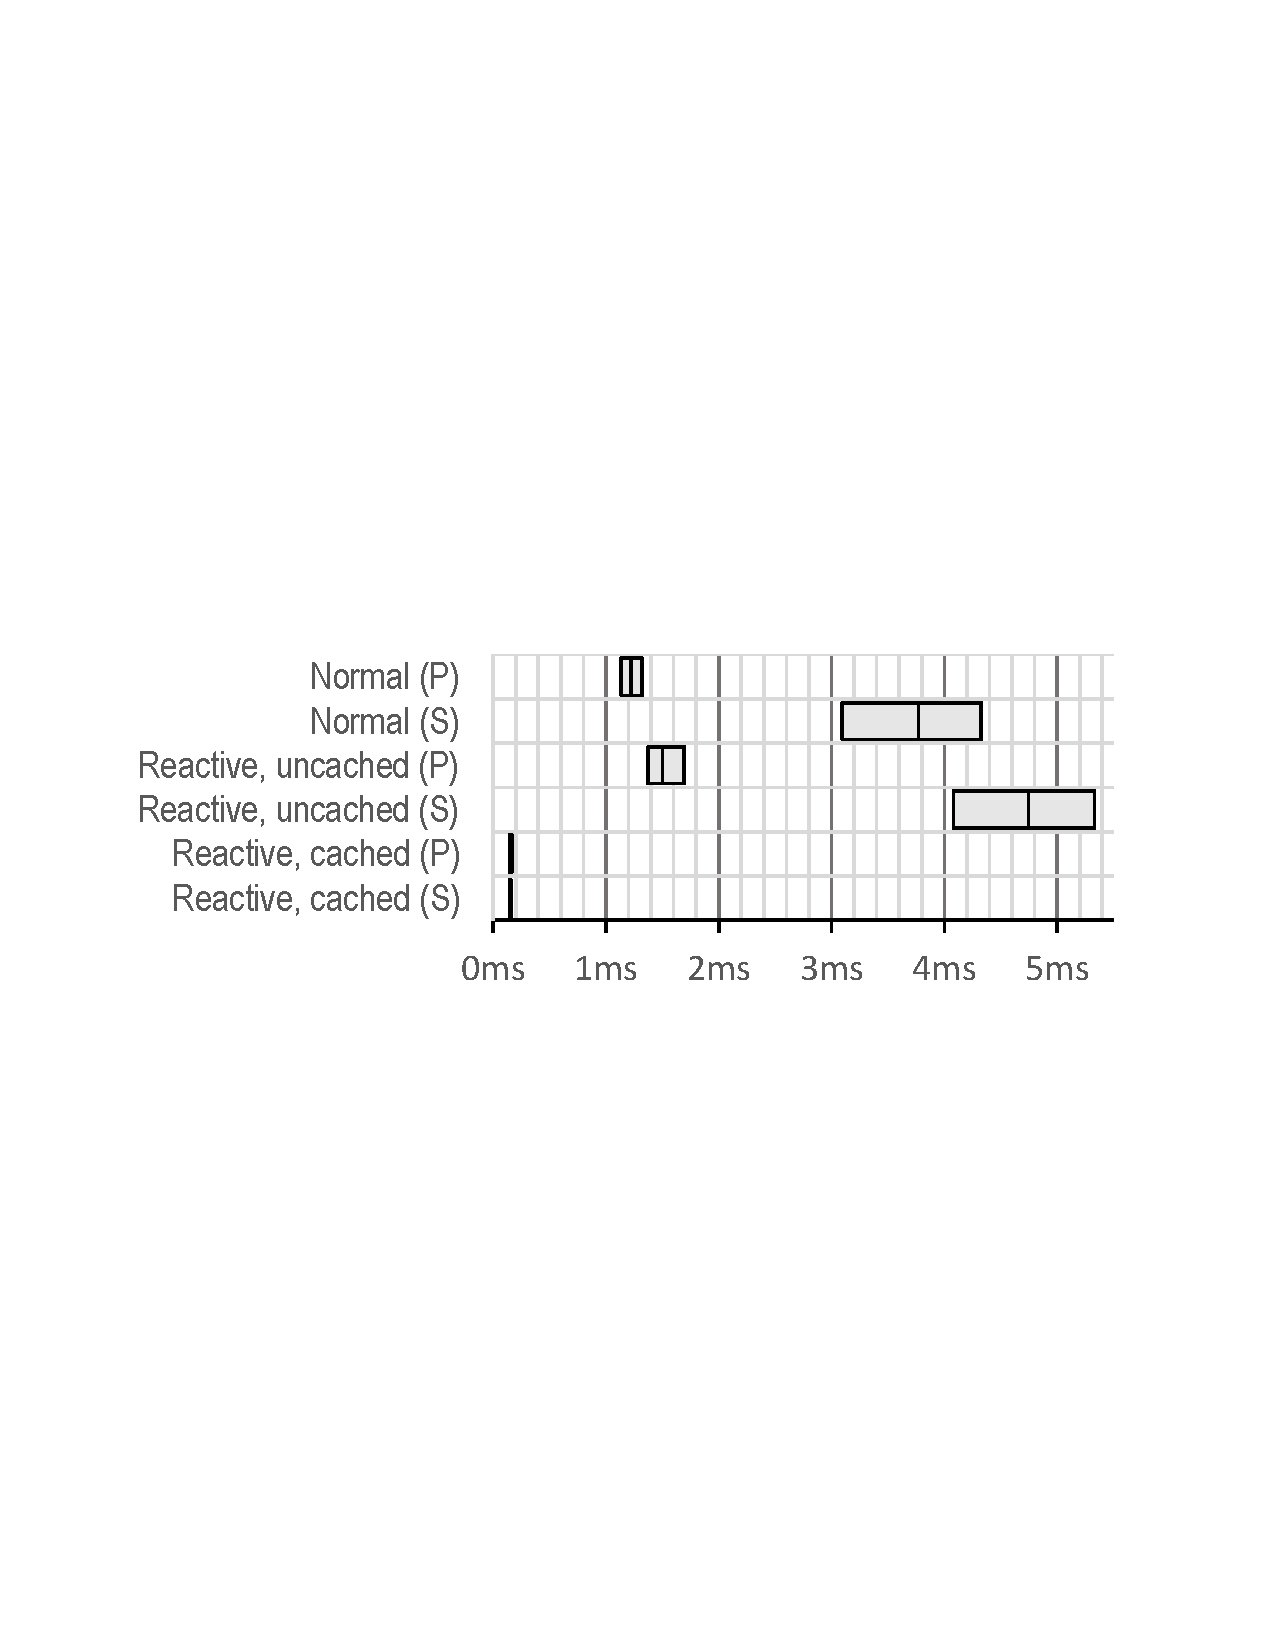
\includegraphics[width=\columnwidth, viewport=67 322 534 477]{figs/query-latencies}\\[.2in]
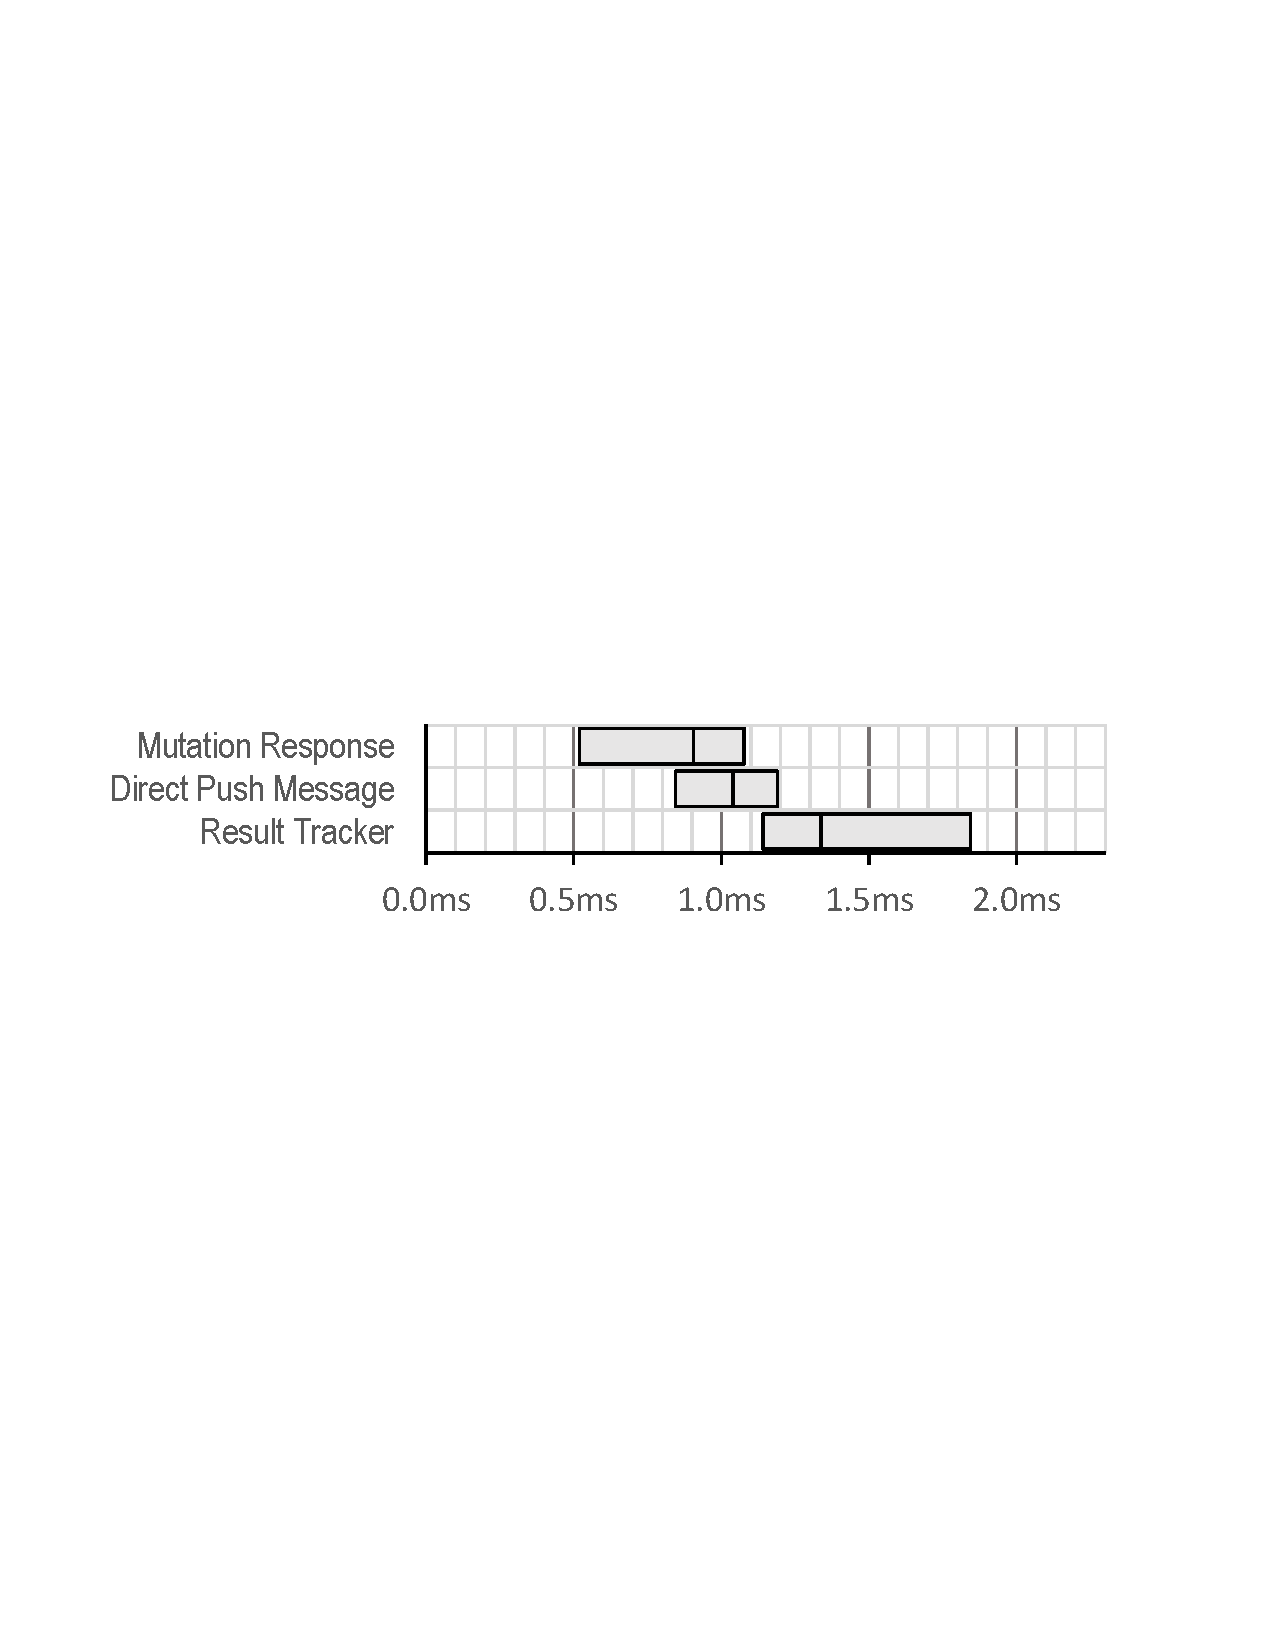
\includegraphics[width=\columnwidth, viewport=54 354 530 444]{figs/push-latencies}\\[.2in]
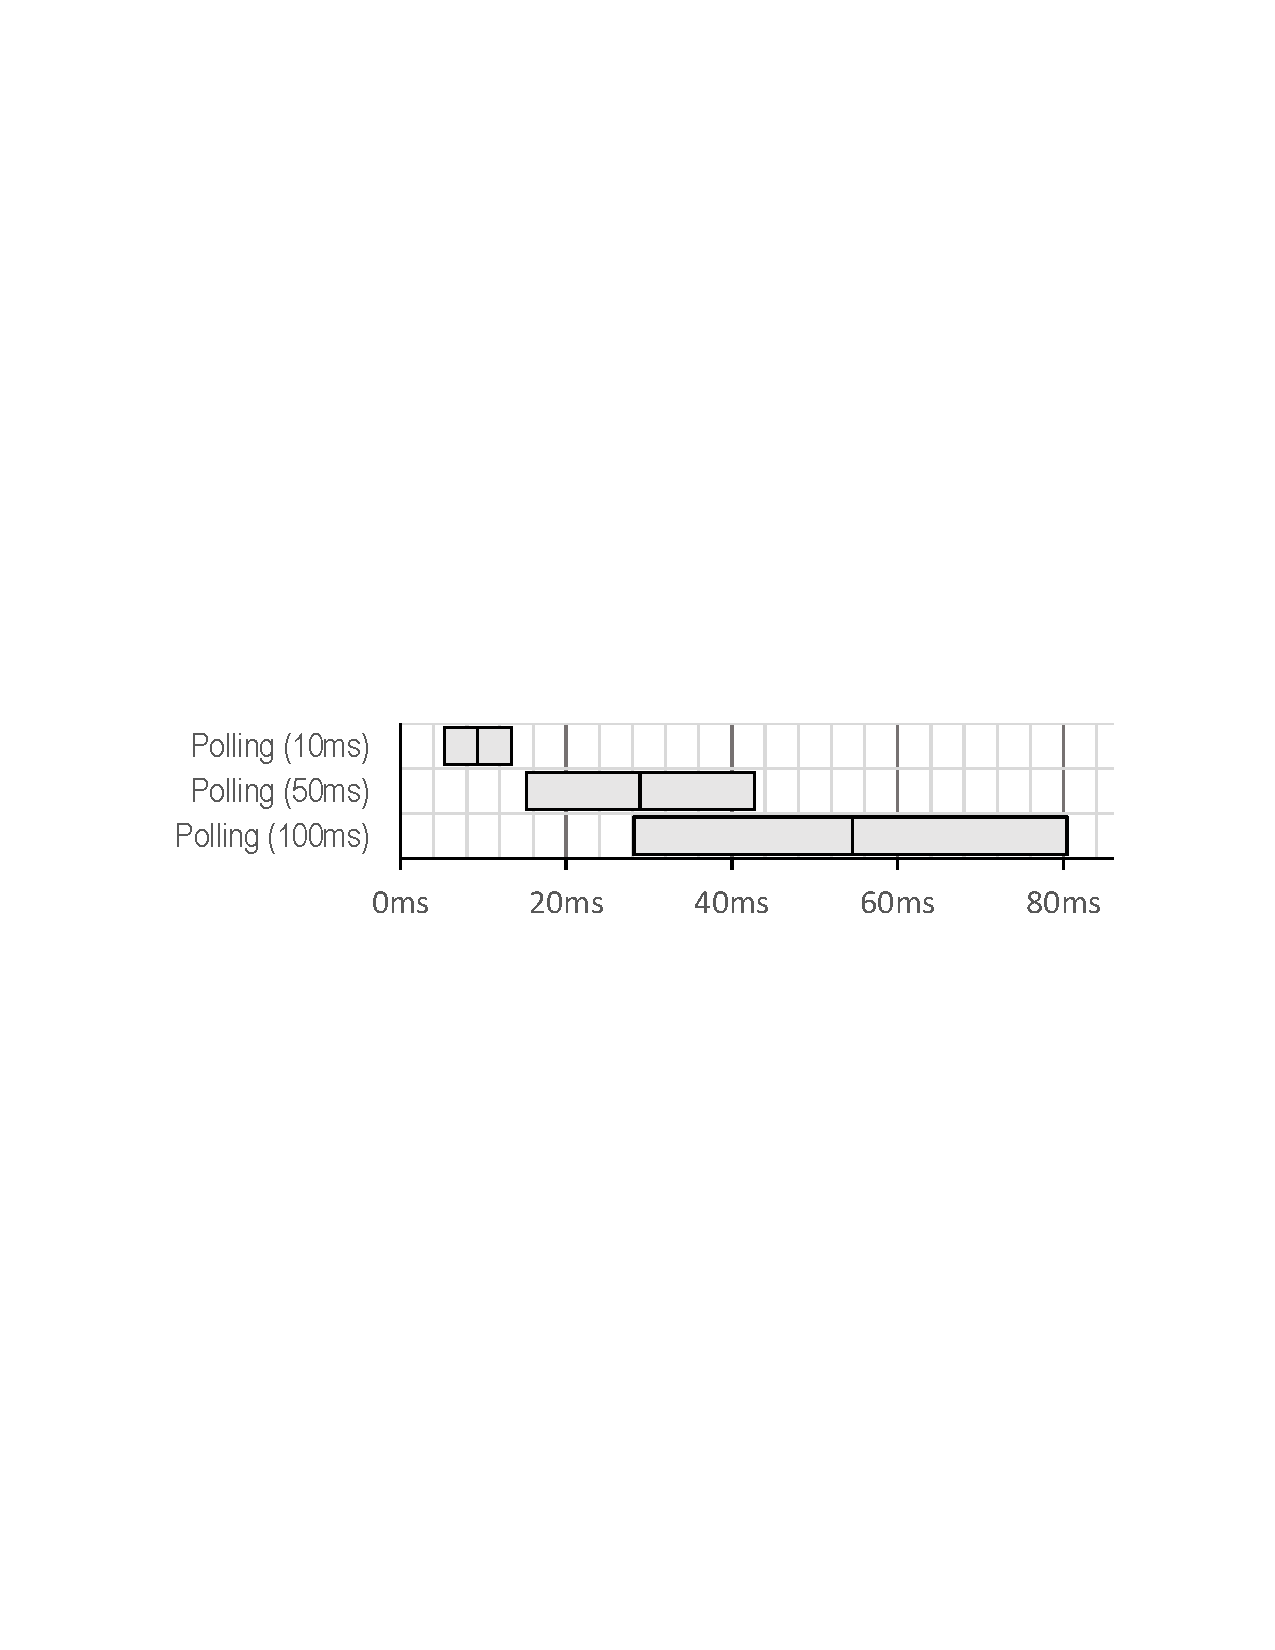
\includegraphics[width=\columnwidth, viewport=85 354 534 444]{figs/polling-latencies}\\
\end{tabular}
\caption{Measured latencies under low load, in milliseconds. The line in the middle of each box is the median, and the left and right edge are the first and third quartile. \textbf{(top)} Latencies for parallel and sequential queries; \textbf{(middle)} latencies for mutation response, application-level propagation using direct messages, and automatic propagation using result trackers; \textbf{(bottom)} propagation latencies for the polling solution at various frequencies.}\label{fig:querylatencies}
\end{figure}

For measuring query latency, we execute a query on a view that calls each of four items (either sequentially or in parallel) to collect some value and returns the values in an array (Fig.~\ref{fig:queries}). We now compare the latency when executed normally (\lstinline|Query|) to the latency when executed as a reactive computation (\lstinline|OneTimeReactiveQuery|). The normal latency for the sequential and parallel versions are shown in the first two rows of Fig.~\ref{fig:querylatencies} (top). The median latency is about 1.2ms for the parallel query and 3.8ms for the sequential query. This is consistent with the round-trip time of a typical grain call taking a bit less than 1ms. For the reactive queries, we distinguish two cases. If  the relevant summaries are not already cached on the silo, the query takes about 25\% longer than normal (rows 2,3). This overhead is caused by the installation and removal of the summary caches, and by scheduling overhead of our reactive caching implementation. However, if summaries for the items are already cached on the silo (for example, if another view is tracking the same items), the latency of \lstinline|OneTimeReactiveQuery| is less than 200$\mu$s (rows 4,5) because remote calls can be completely avoided. 

\paragraph{Conclusions.} The results demonstrate that (1) the latency overhead of constructing the dependency graph is modest, and (2)  the caching effect alone can improve latency, even if not using the reactive features.

\subsubsection{Propagation Latency}

For measuring propagation latency, a view sends an update message to an item it depends on, and measures how much time elapses (a) until it receives the mutation response, and (b) until it receives the change propagation. 

First, we measured the speed of explicit propagation, where each item sends a notification message to all dependent views when mutated. This establishes a lower bound on propagation speed in the Orleans framework. The results show that the propagation message arrives right after the mutation completes: close to 1ms after calling the mutation operation (rows 2,3 of Fig.~\ref{fig:querylatencies} (middle)). This is consistent with the underlying system sending the mutation response message and the propagation message at about the same time. 

Second, we measured the speed of automatic propagation provided by our reactive caching algorithm. In that case, the propagation takes about 300$\mu$s longer (row 3), due to the scheduling overhead of our implementation.

Finally, we looked at the propagation speed of a polling-based solution. Fig.~\ref{fig:querylatencies} (bottom) shows the measured latencies, using a sequential query and various polling intervals. As expected, we see a median propagation time in the neighborhood of half of the polling interval plus the query latency, and a wide inter-quartile distance. However, polling every 100ms is usually not advisable (we show impact of polling on throughput in \S\ref{sec:throughput}). Reasonable polling intervals are more typically between 1 and 30 seconds, with a median propagation speed that is easily three orders of magnitude worse than for explicit or automatic change propagation.  

\paragraph{Conclusions.} The results show that our automatic propagation performs much better than a polling solution, while having the same simple programming model; and is not much slower than explicit change propagation, despite offering the advantage of being fault-tolerant, and much simpler to use.


\subsection{Throughput}\label{sec:throughput}

For the throughput experiments, we generate external load as shown in Fig.~\ref{fig:tp-setup}. The load generator contains up to 2000 robots; each runs a continuous loop that sends requests to the service, either to read a view, or to update an item. The percentage of updates in the mix is configurable. 

\begin{figure}
\centering
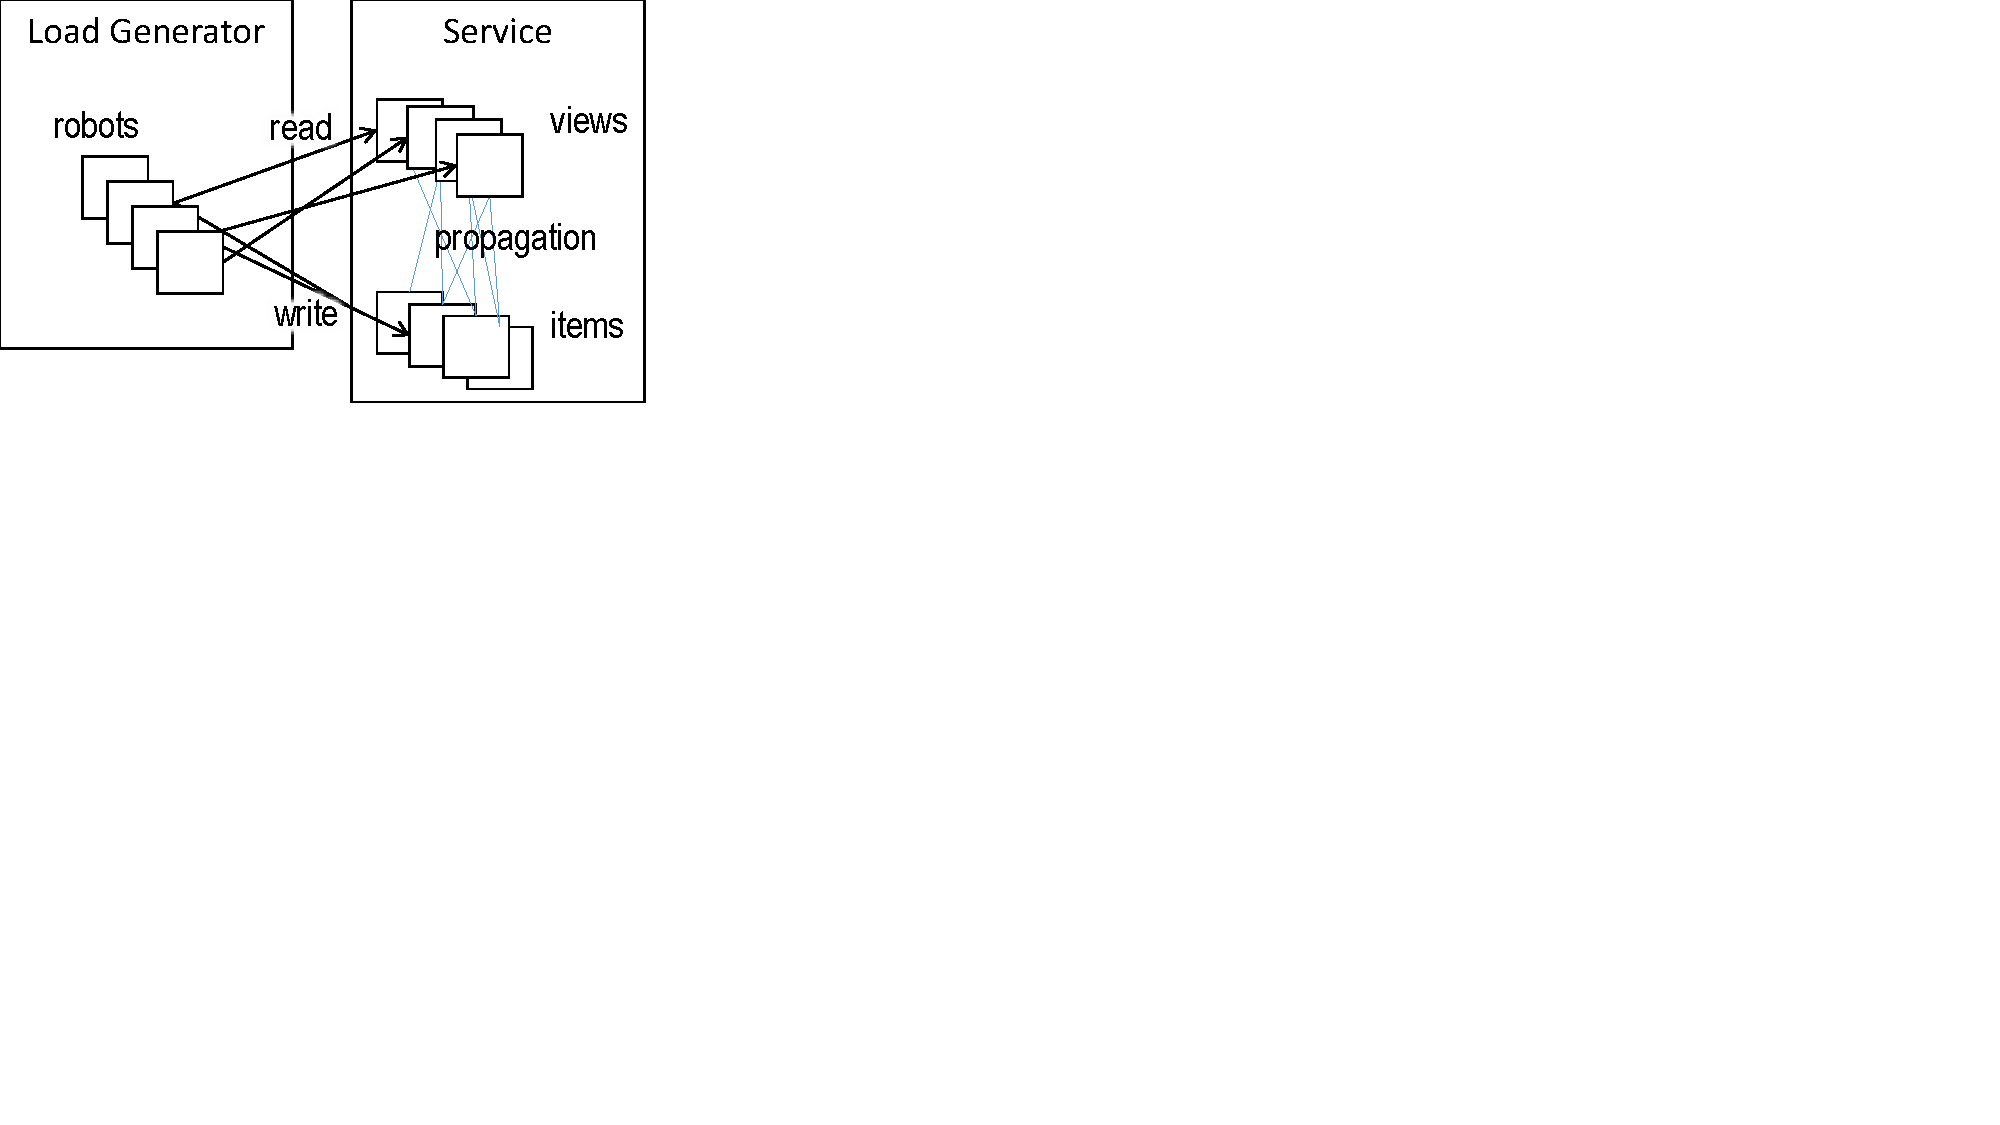
\includegraphics[scale=.5, viewport=0 346 309 540]{figs/tp-setup} 
\caption{Experimental setup for throughput experiments.}\label{fig:tp-setup}
\end{figure}

\begin{figure}
\noindent
\centering
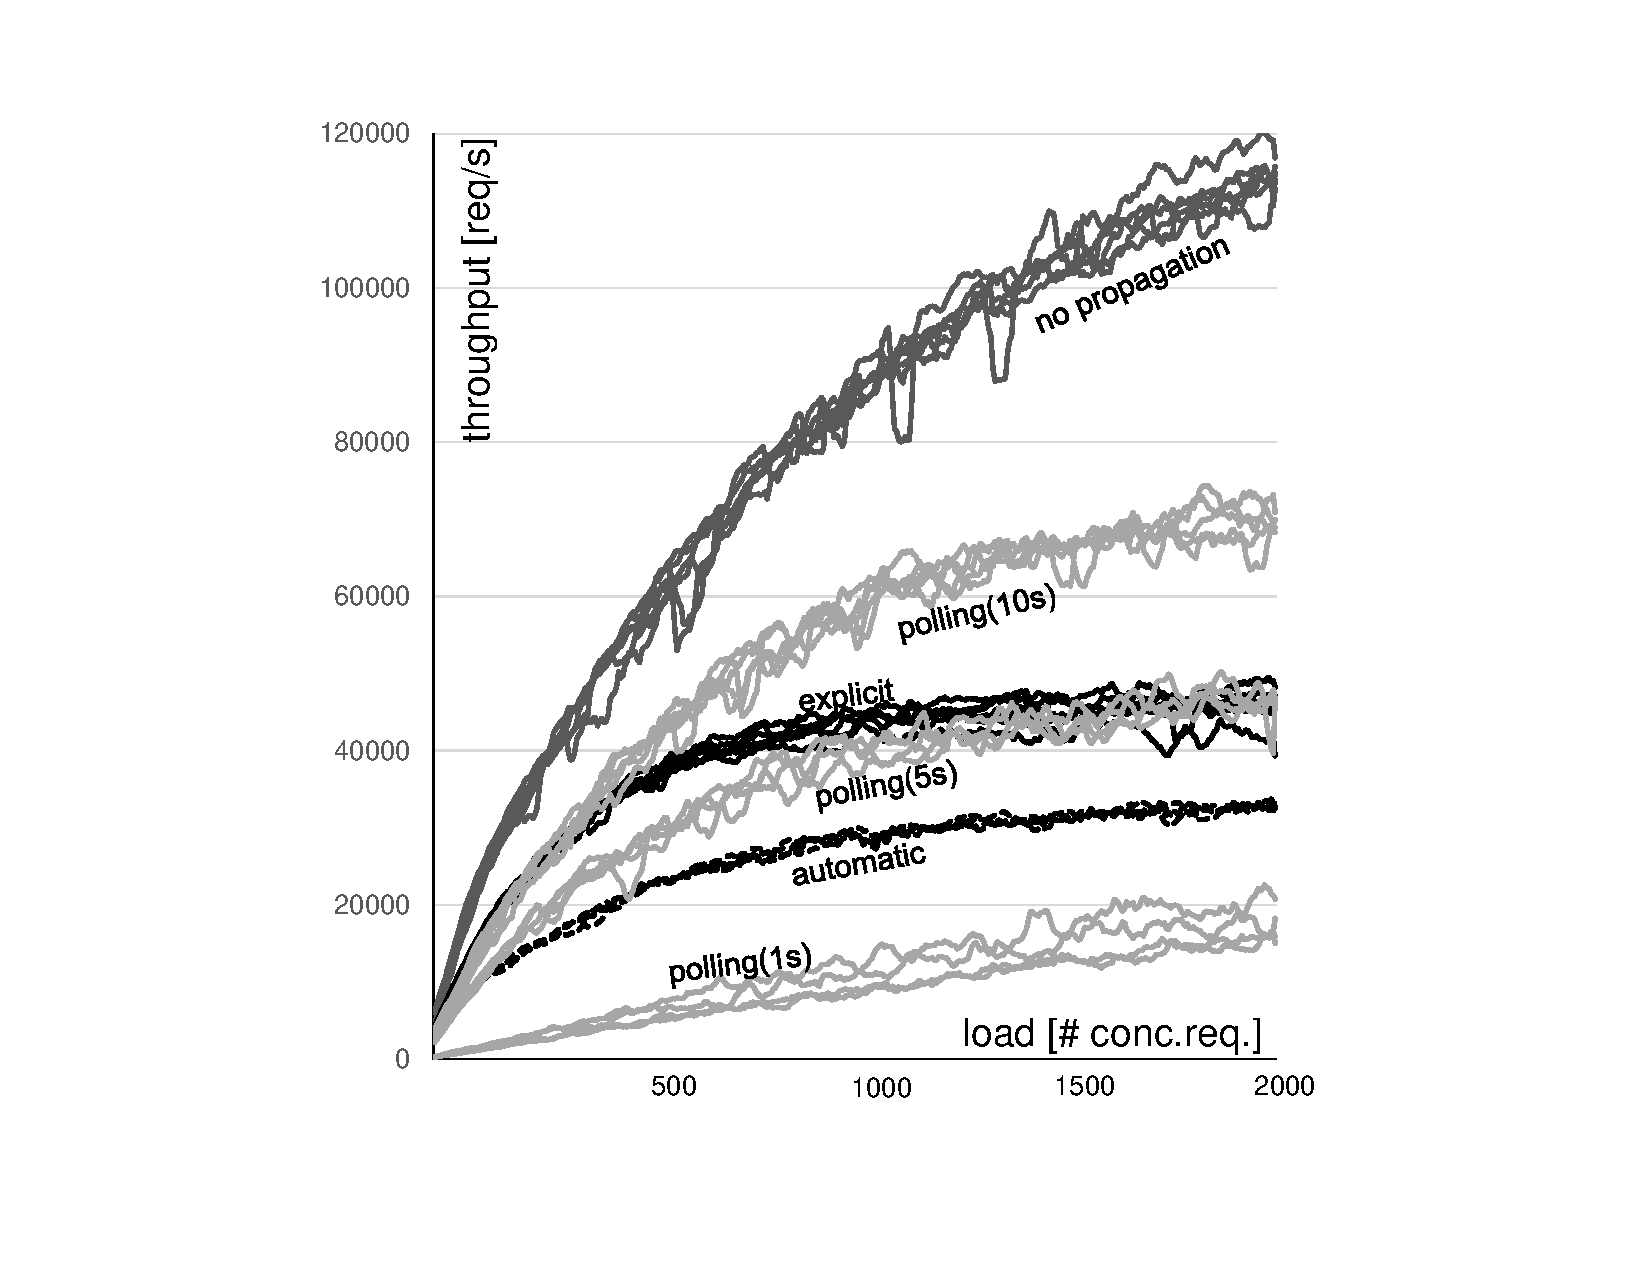
\includegraphics[width=\columnwidth, viewport=154 86 630 553]{figs/tp-curves} 
\caption{Throughput response of different propagation mechanisms, for fanout-20 with 10\% updates.}\label{fig:tp-curves}
\end{figure}
\begin{figure*}
\noindent
\centering
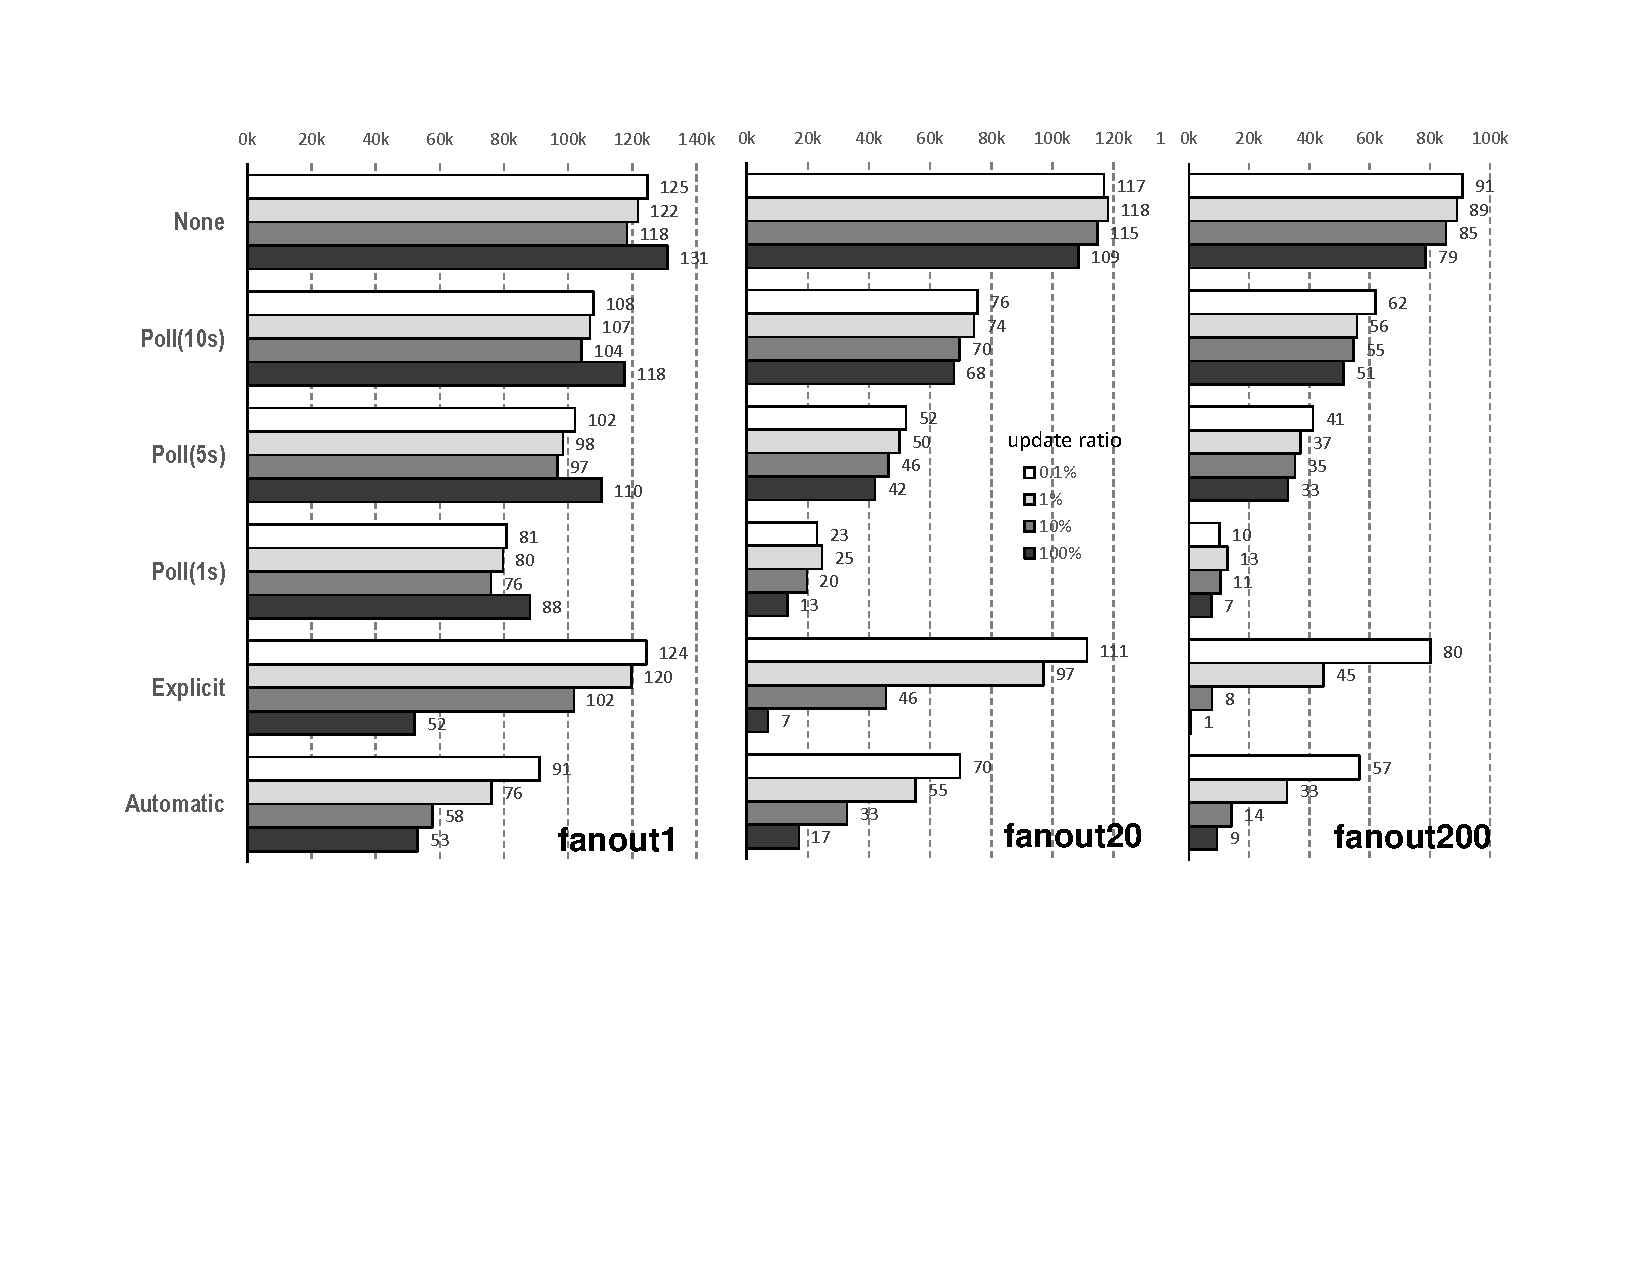
\includegraphics[width=\textwidth, viewport=58 195 726 550]{figs/tp-all} 
\caption{Measured throughput (in thousands of requests per second) for varying configurations (Table~\ref{tab:param}), propagation mechanisms, and percentage of updates.}\label{fig:tp-all}
\end{figure*}

Each experiment gradually increases the robots and measures the throughput over time. The result is a curve that shows how throughput (number of requests handled per second) responds to load (number of requests concurrently in flight). For example, for the \lstinline|fanout20| configuration and a request mix containing 10\% updates, we obtained the curves shown in Fig.~\ref{fig:tp-curves}; each line corresponds to one experiment, and each bundle of similar lines corresponds to several experiments using the same propagation mechanism. 

The best possible throughput is achieved when change propagation is turned off entirely - because all resources are used for handling requests. Here, we reach close to 120k requests per second. But as soon as we use change propagation mechanism, the throughput is lower, because resources diverted to the propagation mechanism: explicit propagation (dotted lines) reaches about 45k, automatic  propagation reaches about 35k. For 10s-polling, the throughput reaches about 70k (better than automatic or manual propagation), but for 1s-polling, it reaches only about 20k (worse than automatic or manual propagation). 

To compare the solutions across different configurations and update ratios, we ran this type of experiment for all combinations, but extended to run fixed load (the maximum number of robots as in Table~\ref{tab:param}) for a while at the end, to measure average  peak throughput for that load. The results are shown in Fig.~\ref{fig:tp-all}. Each column corresponds to a configuration in Table~\ref{tab:param}); each row corresponds to a choice of propagation mechanism; and each bar color corresponds to update percentage. For example, the dark gray bars (10\% updates) in the middle column (fanout20) correspond to the peak throughput in Fig.~\ref{fig:tp-curves}

\mypar{Baseline} With update propagation turned off (top row, labeled \emph{None}), all requests are simple operations on a single grain. We reach a throughput in the neighborhood of  120k for the fanout1 and fanout20 configurations (under a load of 2000 concurrent requests), and near 90k for the fanout200 configuration (under load of 1000 concurrent requests). Though throughput is largely consistent, the numbers show some unexpected variation: throughput degrades somewhat with higher update percentages, and jumps up for the specific combination of fanout1 and 100\% updates). We suspect they are caused by load balancing differences within the Orleans runtime regarding items, views, and requests.

\mypar{Polling} The extra work incurred by polling is (a) inversely proportional to the polling interval, and (b) proportional to the number of items a view depends on. The reduction in throughput (relative to the baseline) is thus modest for views that depend on only 1 item (left column), especially for large polling intervals, but if the view depends on 10 items (middle and right column), the throughput reduction is significant.

\mypar{Explicit Propagation} The extra work incurred by explicit propagation is proportional to both the percentage of updates and the fan-out. The results confirm this: (1) we see o.k. throughput results for update percentages up to 1\%, and (2) we see terribly low throughput for the combination of high fanout and high update percentage, as low as 1k (lowest of all) for fanout200 and 100\% updates.

\mypar{Automatic Propagation} There are two main differences between the work required for automatic and explicit propagation: (1) automatic propagation incurs a bit more work due to scheduling indirection, re-execution of summaries, and management of reactive caches;  and (2) automatic propagation can adapt to back-pressure and reduce the number of updates sent.  We can observe these effects: throughput for automatic propagation is generally lower than for explicit propagation, except for high update rates and/or fanout where explicit propagation suffers more. 
 
\mypar{Conclusions} The results show that automatic propagation is generally competitive with explicit propagation, despite the added benefit of fault tolerance and a simpler programming model. It is even better in cases where there are many updates to be propagated, thanks to its batching optimization. Polling remains an acceptable solution for applications that do not require quick propagation time; it can be tuned to reliably consume little resources, even under high update rates.

 
 



\section{Related Work}

As discussed in the introduction, reactive programming is a rich area of research that spans language design, algorithms and implementation architecture (see the survey \cite{reactivesurvey}).

A main difference between our solution and much prior work on FRP \cite{frp-firstprinciples,frp-animation,frp-frtime,elm,afp} is that our computations are not expressed using a set of operators/combinators supported by the compiler, but execute like regular code of the host language (imperative, object-oriented C\#). Incrementality is achieved at runtime, by decomposing the computation into subcomputations at that can be selectively re-evaluated if their dependencies change. In that sense, our solution follows the same principle as self-adjusting computation \cite{acar-ahmed-blume-POPL08,Acar:SelfAdjustingExperiments,Acar:SelfAdjustingOverview,Hammer:Ceal09,Acar:SelfAdjustingTypes10}, one-way dataflow constraints \cite{camil}, or incremental concurrent revisions \cite{burckhardt-leijen-yi-sadowski-ball-OOPSLA11}, except that here, we use the encapsulation afforded by the actor model as a means to decompose the computation.


Change propagation is semantically subtle. In sychronous models, time is explicit. Asynchronous models may make strong consistency guarantees based on some form of version tracking, or may have weaker consistency guarantees. For example, a so-called glitch means that an observer sees two observables A, B that have inconsistent state, meaning that the set of updates propagated to A is different from the set of updates propagated to B. Many reactive systems strive to eliminate glitches (e.g. using topological ordering of dependencies), but some embrace them.

Clearly, how to best balance consistency and performance is highly dependent on the architecture and workload. 
avoiding glitches in a distributed actor system like ours is likely to add significant latency overhead: updates are only partially ordered to begin with, and dependencies are detected dynamically. Also, for the applications we have in mind, it is typically preferrable to quickly display a glitchy result and then quickly correct it, than to generally wait longer. Consequently, we chose an algorithm that does not avoid glitches or causality violations categorically, but guarantees that they are ephemeral (\S\ref{sec:cp}). This tradeoff is quite similar to the variations of eventual consistency.
 

\subsection{Expressing Views.} Often, views can observe other views, creating a directed acyclic graph of dependencies. How to express such dependency graphs using recursive operators is a key question in the area of dataflow languages, functional reactive programming, and object-oriented frameworks such as Rx. In relational database systems, views are expressed by relational queries (which allows changes to be propagated incrementally). in Facebook's react.js, the application state is observed by a tree-structured virtual DOM, which is in turn observed by the browser's DOM. And in relational database systems, views are expressed by relational queries (which allows changes to be propagated incrementally)

 


 
 
\cite{burckhardt-leijen-yi-sadowski-ball-OOPSLA11}
\cite{camil}


\cite{alive}
\cite{react}

\cite{elm} language for gui construction

\cite{statelines} inverse problem

% These are just paragraphs of information about certain topics, still needs to be put in a nice text if they are used %


% RP %
\paragraph{General purpose FRP models} \cite{reactivesurvey} require you to write down your program in terms of signals and behaviours, i.e. explicitly write down the dependency graph. Furthermore, while still a lot of research is being conducted to efficiently perform glitch-free propagation cycles on a single node, lately some initial research is being performed to do this in a distributed setting \cite{elm}\cite{drescala}. Even though future research might solve this, it is still an open research question on how to maintain a distributed propagation algorithm that can handle dynamic dependency graphs and doesn't require a central coordinator. Yet, these two properties are essential to providing scalable services, since topologies change, nodes fail and coordination is very costly.

The presented model in this paper is very different in the sense that (1) the programmer is not required to explicitly provide the dependency graph using special constructs/types (2) because it allows executions that observe a glitch. Yet, it does guarantee that it will eventually perform a glitch-free execution. As a result, this algorithm naturally lends itself more towards large-scale, fault-tolerant systems, by sacrificing some consistency guarantees. At the same time it demands less from the programmer. \newline


%% More info on distributed FRP %%
Citations straight from \cite{drescala}:

\emph{We propose Distributed REScala, a reactive language
with a change propagation algorithm that works without
centralized knowledge about the topology of the dependency
structure among reactive values and avoids unnecessary
propagation of changes, while retaining safety guarantees
(glitch freedom).}

The ``centralized knowledge of the topology of the dependency structure'' is very important here. This doesn't mean they don't need a central coordinator, because then on page 7 you can find the crux of why I think the algorithm is being oversold:

\emph{Update turns in SID-UP must happen mutually exclusive:
Concurrent updates may cause glitches by exposing partial
results to each other whenever they affect the same node in
the DG. If this can not be guaranteed by the nature of the
application, a centralized coordinator is needed during the
admission phase. Every thread that wants to admit a change
must first contact this coordinator to acquire exclusive access
to execute an update turn. After the turn completes, the
exclusive access is relinquished to allow the next update turn
to start. These are the only two messages outside of regular
pulses in SID-UP and they require many-to-one communication
only. Supporting concurrent update turns, thus getting
rid of the centralized coordination, is ongoing work.}


% Big Data %
\paragraph{Big data processing/analytics models.} Two types: (1) batch processing (Spark, Hadoop) \cite{mapreduce} and (2) stream processing (Apache Flink \& Storm). Can be seen as a  distributed FRP model, because it uses functional operators over sets of distributed data. Batch processing assumes the data doesn't change and stream processing is able to handle continuously changing data. They have the same drawback as any FRP, in that they require special purpose types and functions.


\paragraph{Dataflow (Synchronous) Languages}
\cite{syncdataflow}
The main idea is that they describe, and formalize, dataflow sychronous languages and categorize two important types of applications w.r.t. asynchronous environments: "exochronous" and "endochronous". Exochronous applications can have multiple inputs to the dependency graph, while endochronous only have one. As a consequence, synchronous endochronous applications can be easily compiled into an asynchronous setting, i.e. distributed application, without coordination. Exochronous applications on the other hand require a coordinator when distributed. \newline

Haven't read this paper very well, but one of my friends at the lab his paper about a distributed reactive propagation algorithm got rejected because he did not mention it...
It's a pretty terse paper, but if you're interested, the crux about the compilation to asynchronous environments is on page 141 (or 17 in de pdf), it's in the related folder. I'm not sure if and how we should incorporate this though. \newline

\cite{esterel} In multi-clock Esterel different parts of the program are no longer bound to the global clock. This means that we could possibly run different parts of the reactive program in a distributed setting. Nevertheless, the model assumes instantaneous communication between the parts running on different clocks and clock ticks happen mutually exclusive. This inherently makes it a bad fit for implementing scalable distributed services.


\cite{orleans}

\section{Conclusion}

We have motivated, explained, implemented, and evaluated a new mechanism called \emph{reactive computations} that makes it easier for developers of actor-based services to quickly and easily propagate changes in actor states to clients that depend on it. Our results show that even though its API is as simple as polling, our fault-tolerant distributed reactive caching algorithm can propagate changes fully automatically and very efficiently. Therefore, it is an attractive alternative to complex and error-prone solutions based on observer patterns, with explicit change propagation at the application level.

Much work remains to be done. We believe the peformance of our implementation can be further improved, by identifying hotspots and improving the scheduler. Also, we would like to gather more experience in an industrial context; we have already started a collaboration with a game developer team. Moreover, we would like to explore how to combine reactive computations with other mechanisms, such as streams and event sourcing. Finally, we are working on formalizations for describing the virtual actor model, the reactive caching algorithm, and the consistency guarantees.
 

 

\acks

Acknowledgments, if needed.

% We recommend abbrvnat bibliography style.

\bibliographystyle{abbrvnat}

% The bibliography should be embedded for final submission.

\bibliography{citations}


\end{document}
